\section{Efficiencies}
\label{sec:eff}

The lack of simulated samples at every conceivable point in the $(m_\db, \tau_\db$) plane means
that the points that are available must be used to interpolate (and extrapolate) to all regions.
Assuming that the efficiencies vary continuously, it is possible to parameterize efficiencies using
spline interpolation.
This is done by pararameterizing the way that efficiency varies with mass and lifetime.

The efficiency due to the \lhcb acceptance region is stable as a function of mass, but does vary
slightly with mass, from \approx$18\pc$ for a $\mass{\db}=214\mev$ sample, to \approx$15\pc$ for a
$\mass{\db}=4000\mev$ sample.


\subsection{Reconstruction and stripping}
The reconstruction and stripping efficiencies are obtained from simulation and given in
\Tab{tab:eff:summary}.
Samples generated with larger lifetime have lower efficiencies because the Dark
Bosons will increasingly decay outside of the \velo.
This is also the case for low $m(\db)$, where there is a larger boost.
The evolution of the total efficiency as a function of mass (for the $100\ps$ samples) is shown in
\Fig{fig:eff:spline}.



%%mass |  tau |      reco |   trigger |    sel   |    BDT   |    TOTAL
%%2500 |   10 |     10.13 |     75.45 |    70.46 |    84.27 |     4.54
%%2500 |  100 |      3.21 |     67.61 |    70.58 |    83.79 |     1.28
%%2500 | 1000 |      0.40 |     64.38 |    70.53 |    85.26 |     0.15



\begin{figure}
  \begin{center}
    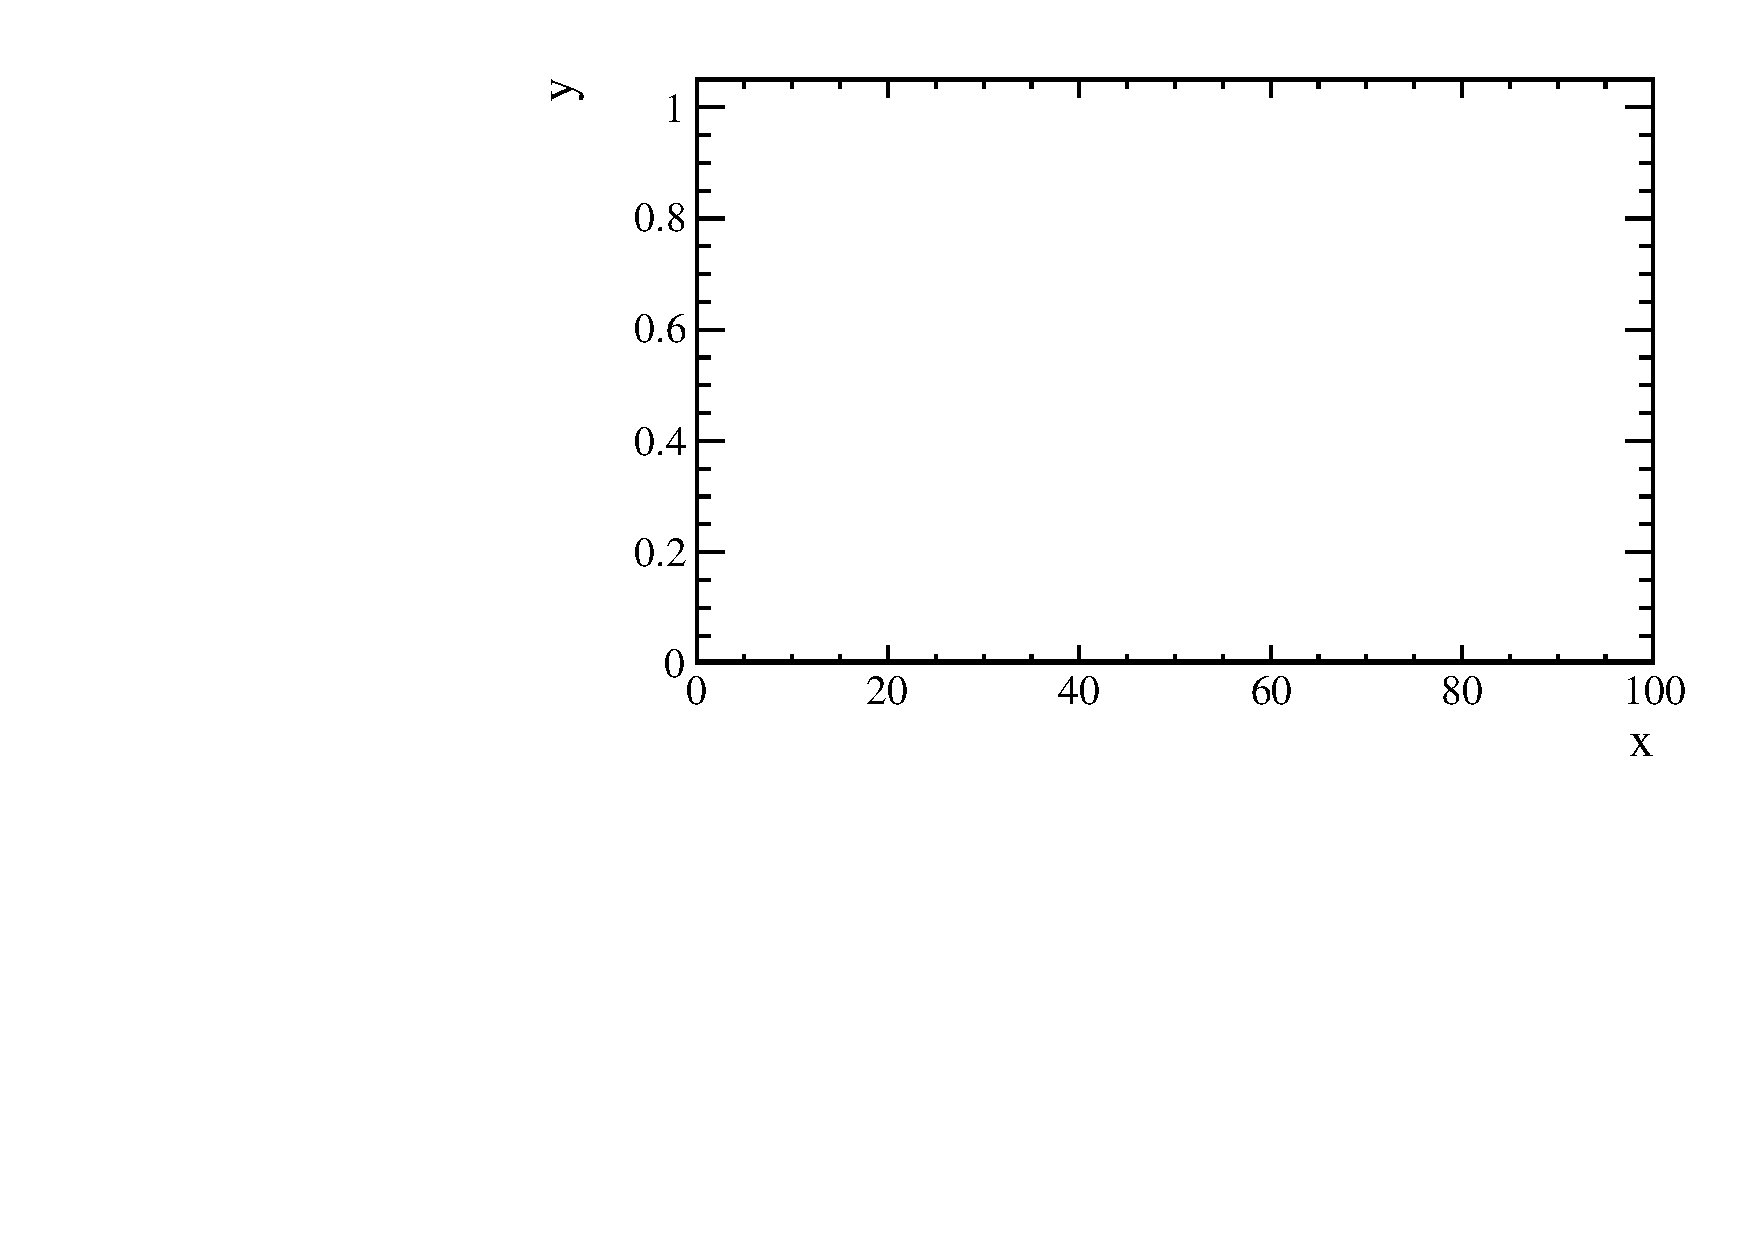
\includegraphics[width=0.48\textwidth]{blank}
    \caption{
      Evolution of the total efficiency, as given in Table~\protect\ref{tab:eff:summary}, where the
      black points indicate the sampled masses, and the red line is the interpolated cubic spline
      intersecting each point.
    }
    \label{fig:eff:spline}
  \end{center}
\end{figure}

%\subsection{Normalization channel}
%The normalization channel is restricted in \qsq region, between 1.1 and $6.0\gevgev$.
%Using generator level simulation, it is determined that $(20.11\pm0.06)\%$ of generated events lie
%in this region.





%\subsection{Lifetime resolution}
%%The lifetime resolution (defined as $\Delta\tau=\tau^\mathrm{meas}_{\db}-\tau^\mathrm{true}_{\db}$)
%%varies as a function of $m_{\db}$, as shown in Fig~\ref{fig:taures:zoom}.
%The lifetime resolution is obtained by fitting
%$\Delta\tau=\tau^\mathrm{meas}_{\db}-\tau^\mathrm{true}_{\db}$, as shown in
%Fig~\ref{fig:taures:zoom}, and finding the $3\simga$ limits of these
%probability density functions.
%For $m_{\mu\mu} > 250\mev$ the $\tau$ measurement is unbiased and has nearly uniform resolution.
%However, for dimuon masses close to threshold, where the break up momentum is small, the lifetime measurement is biased and less precise.
%There is a strong difference between the resolution in the  214 and the 250\mev samples (see
%Fig~\ref{fig:taures:zoom}).  For this
%reason, small samples of simulated signal events were produced at 220 and 235\mev to aid with the understanding of the detector response in this dimuon mass region.

%\begin{figure}
  %\begin{center}
    %%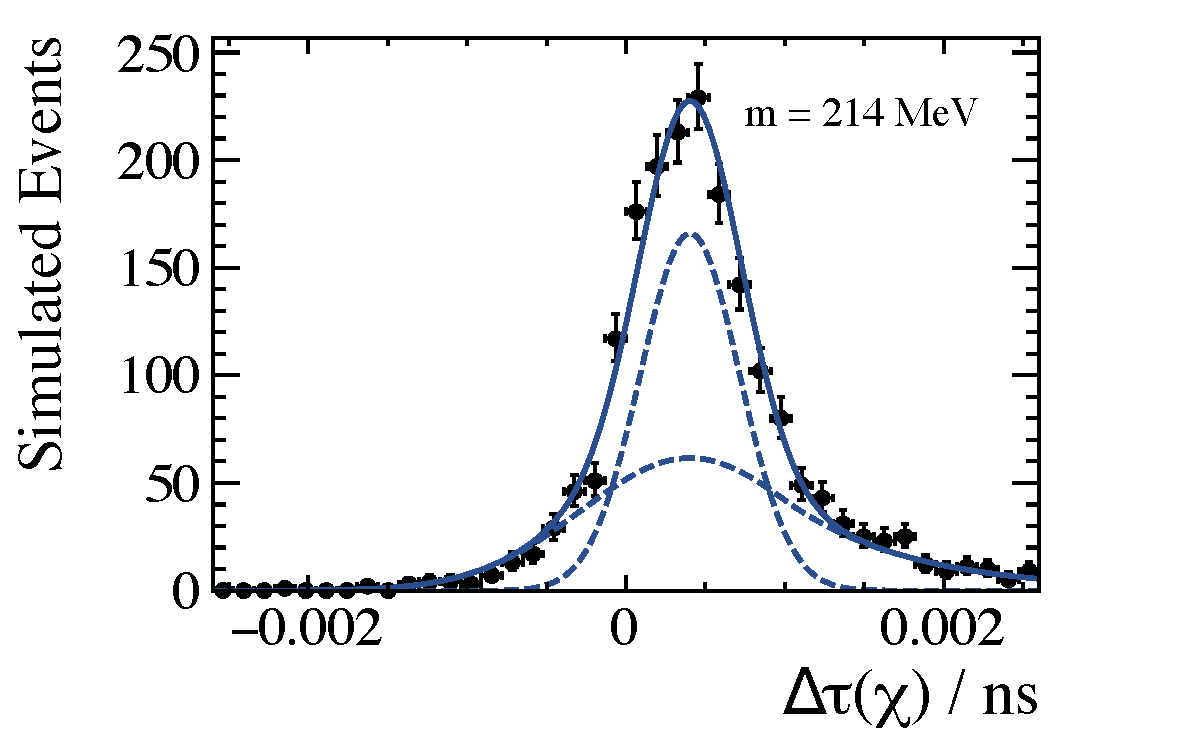
\includegraphics[width=0.42\textwidth]{anaTauResZoom_214}
    %%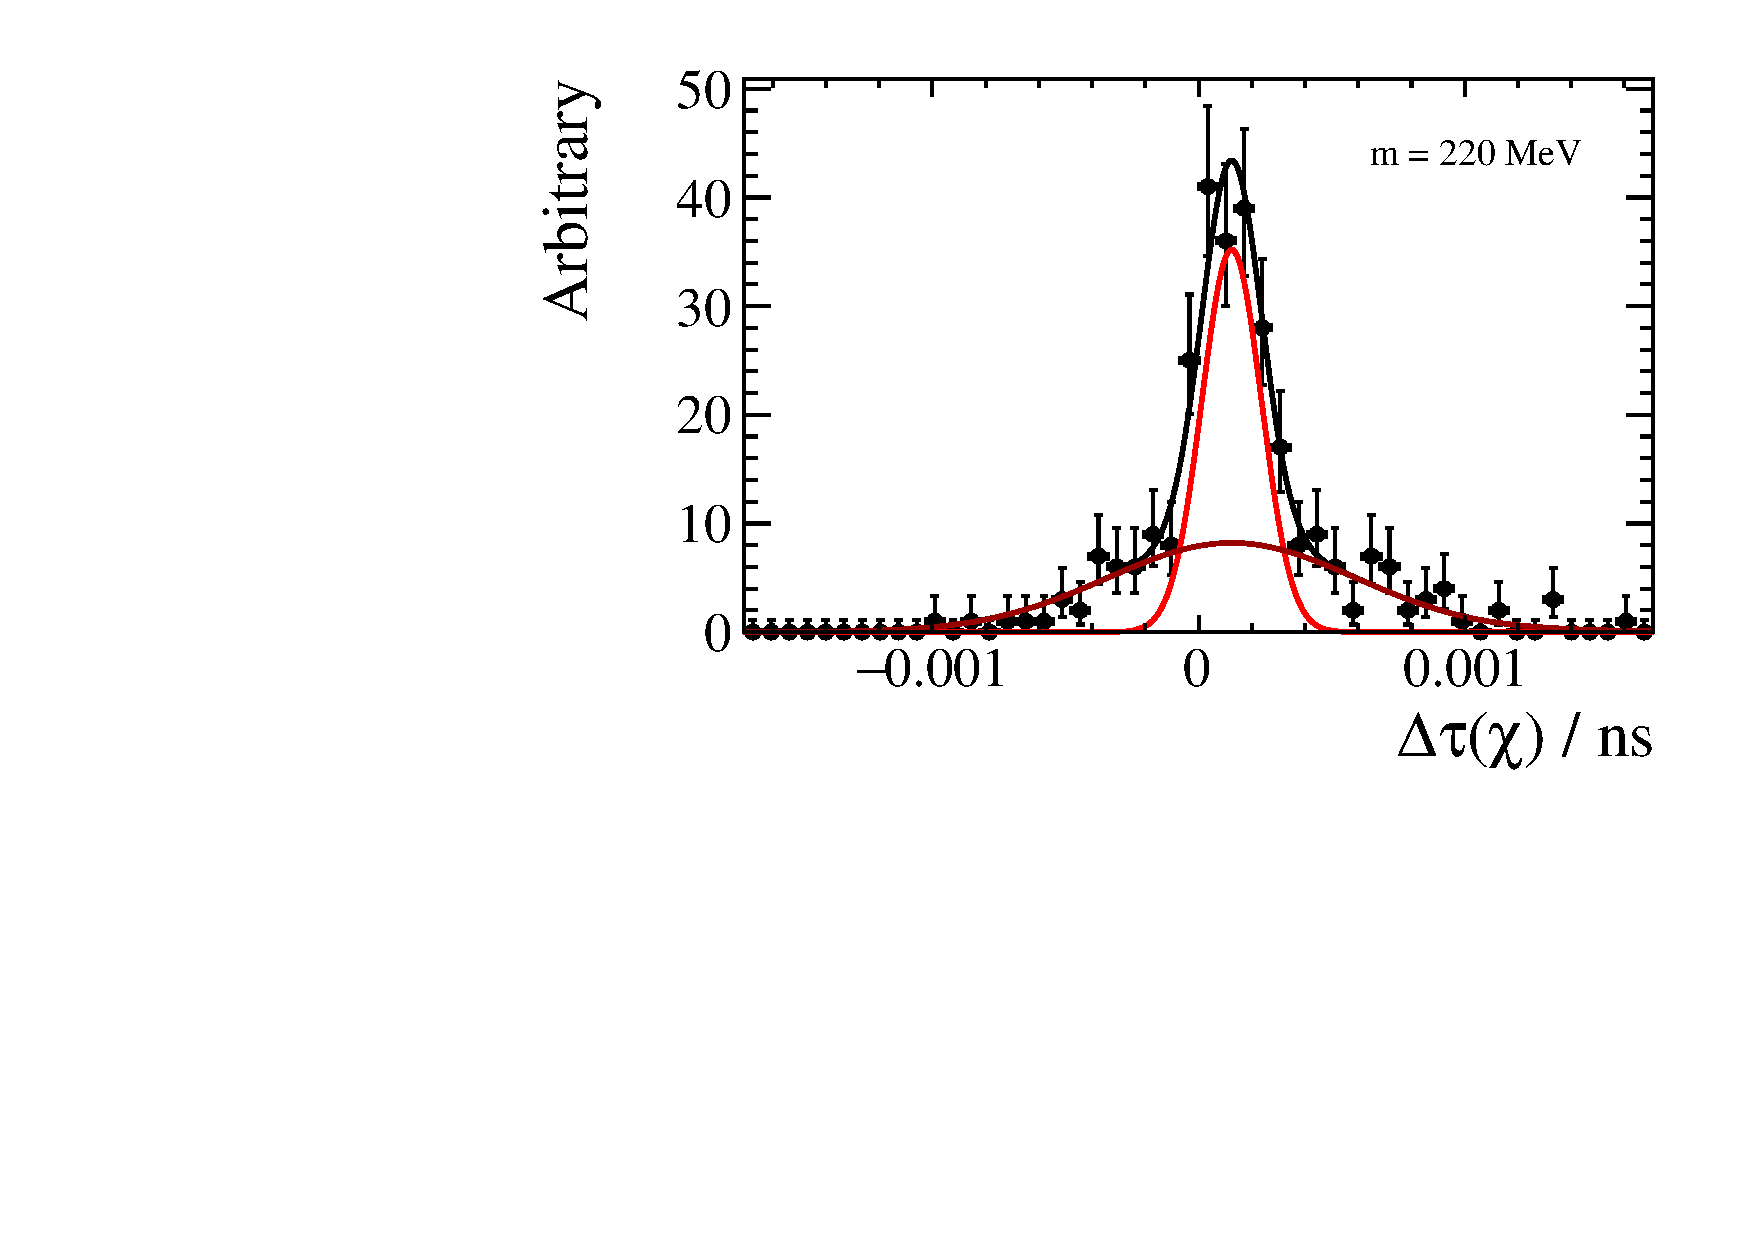
\includegraphics[width=0.42\textwidth]{anaTauResZoom_220}
    %%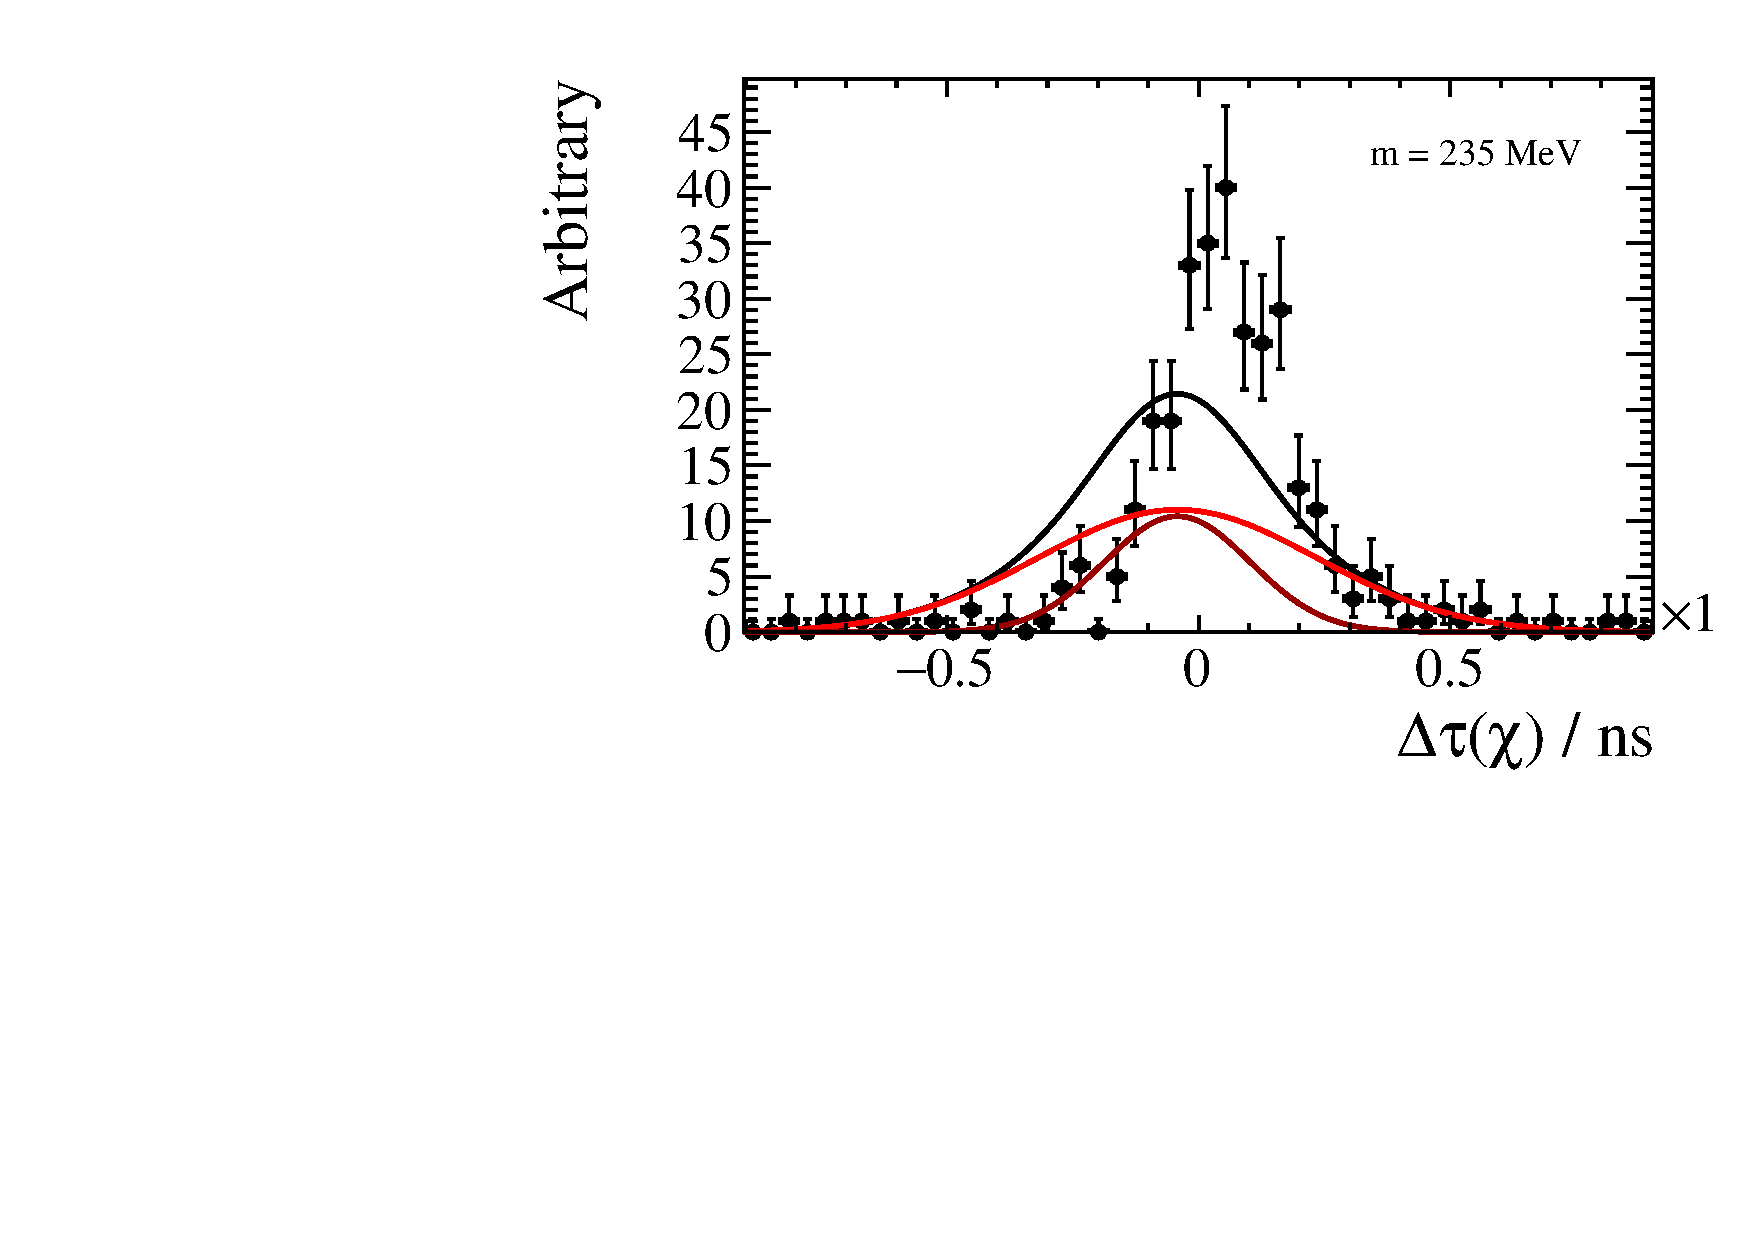
\includegraphics[width=0.42\textwidth]{anaTauResZoom_235}
    %%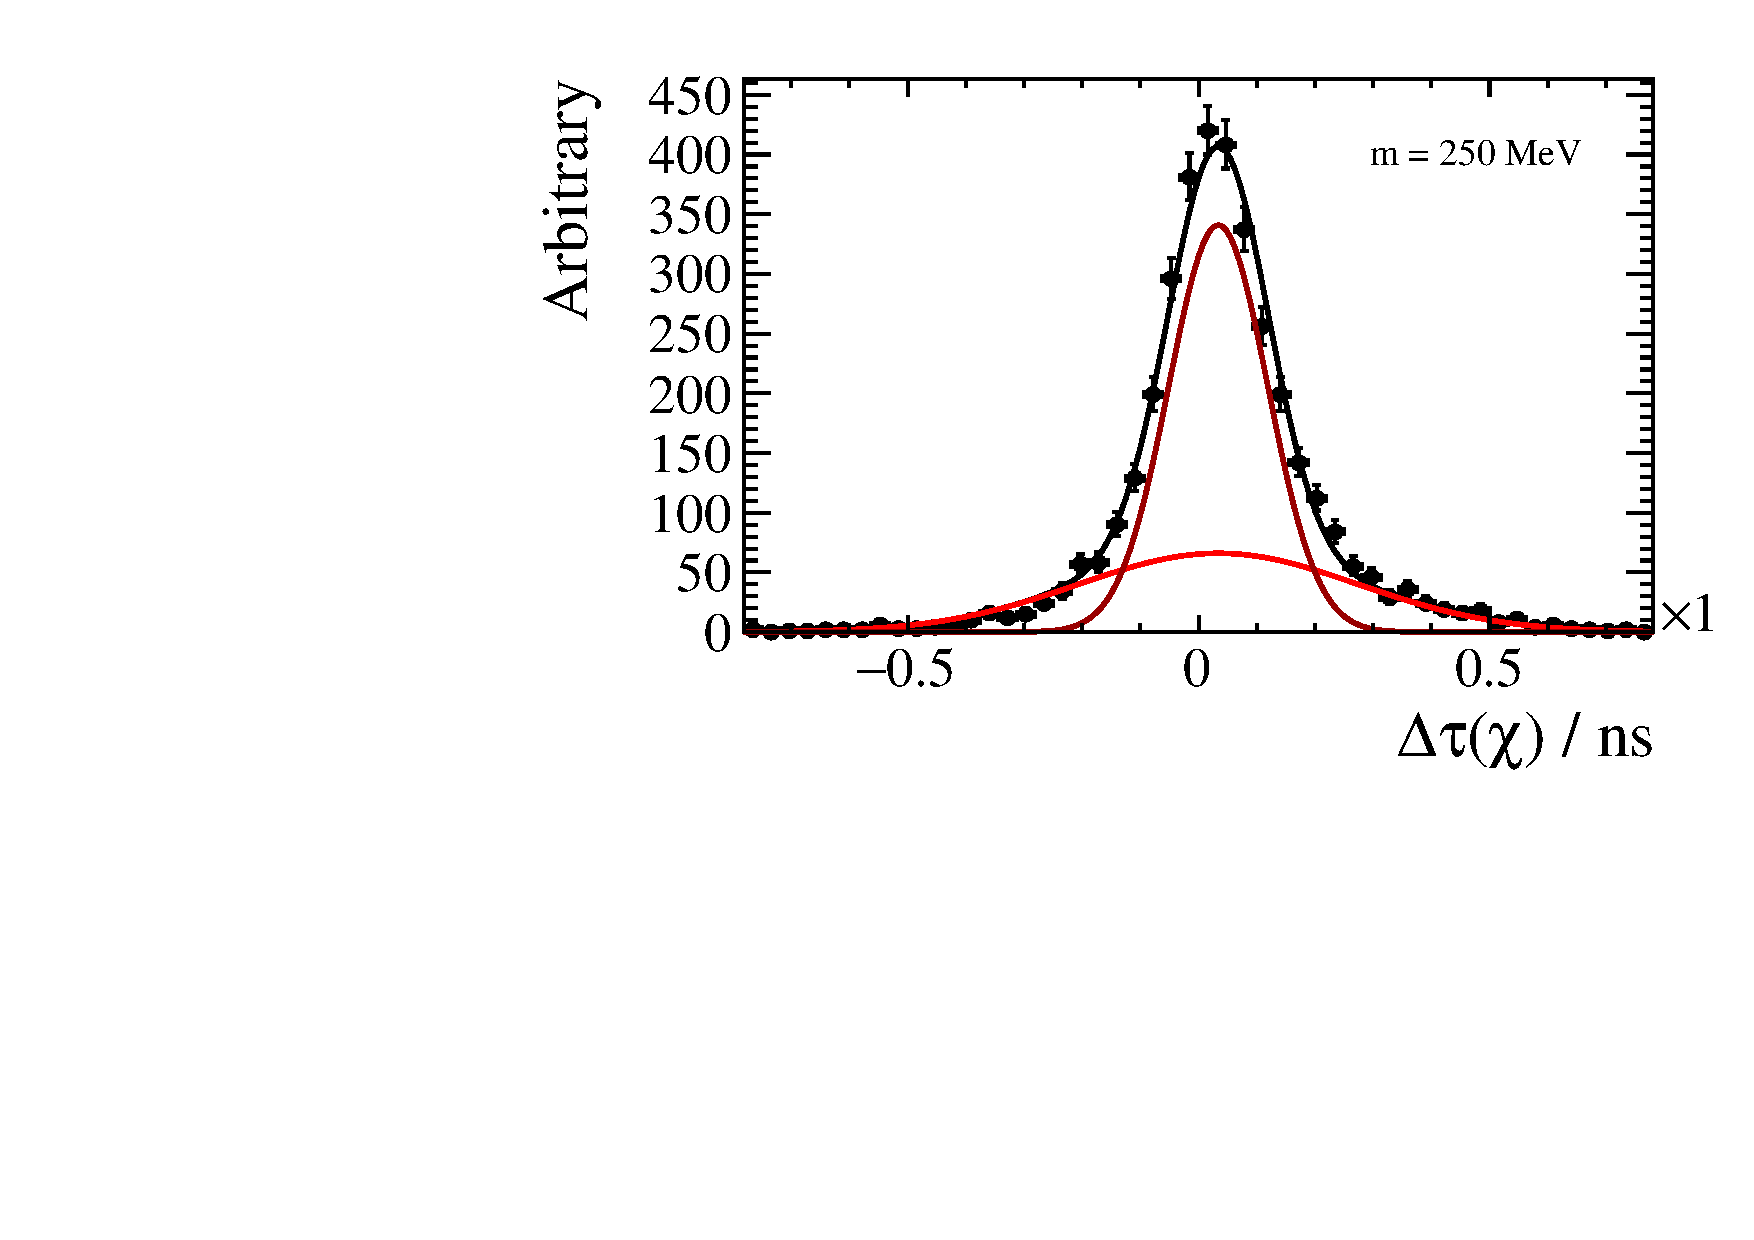
\includegraphics[width=0.42\textwidth]{anaTauResZoom_250}
    %%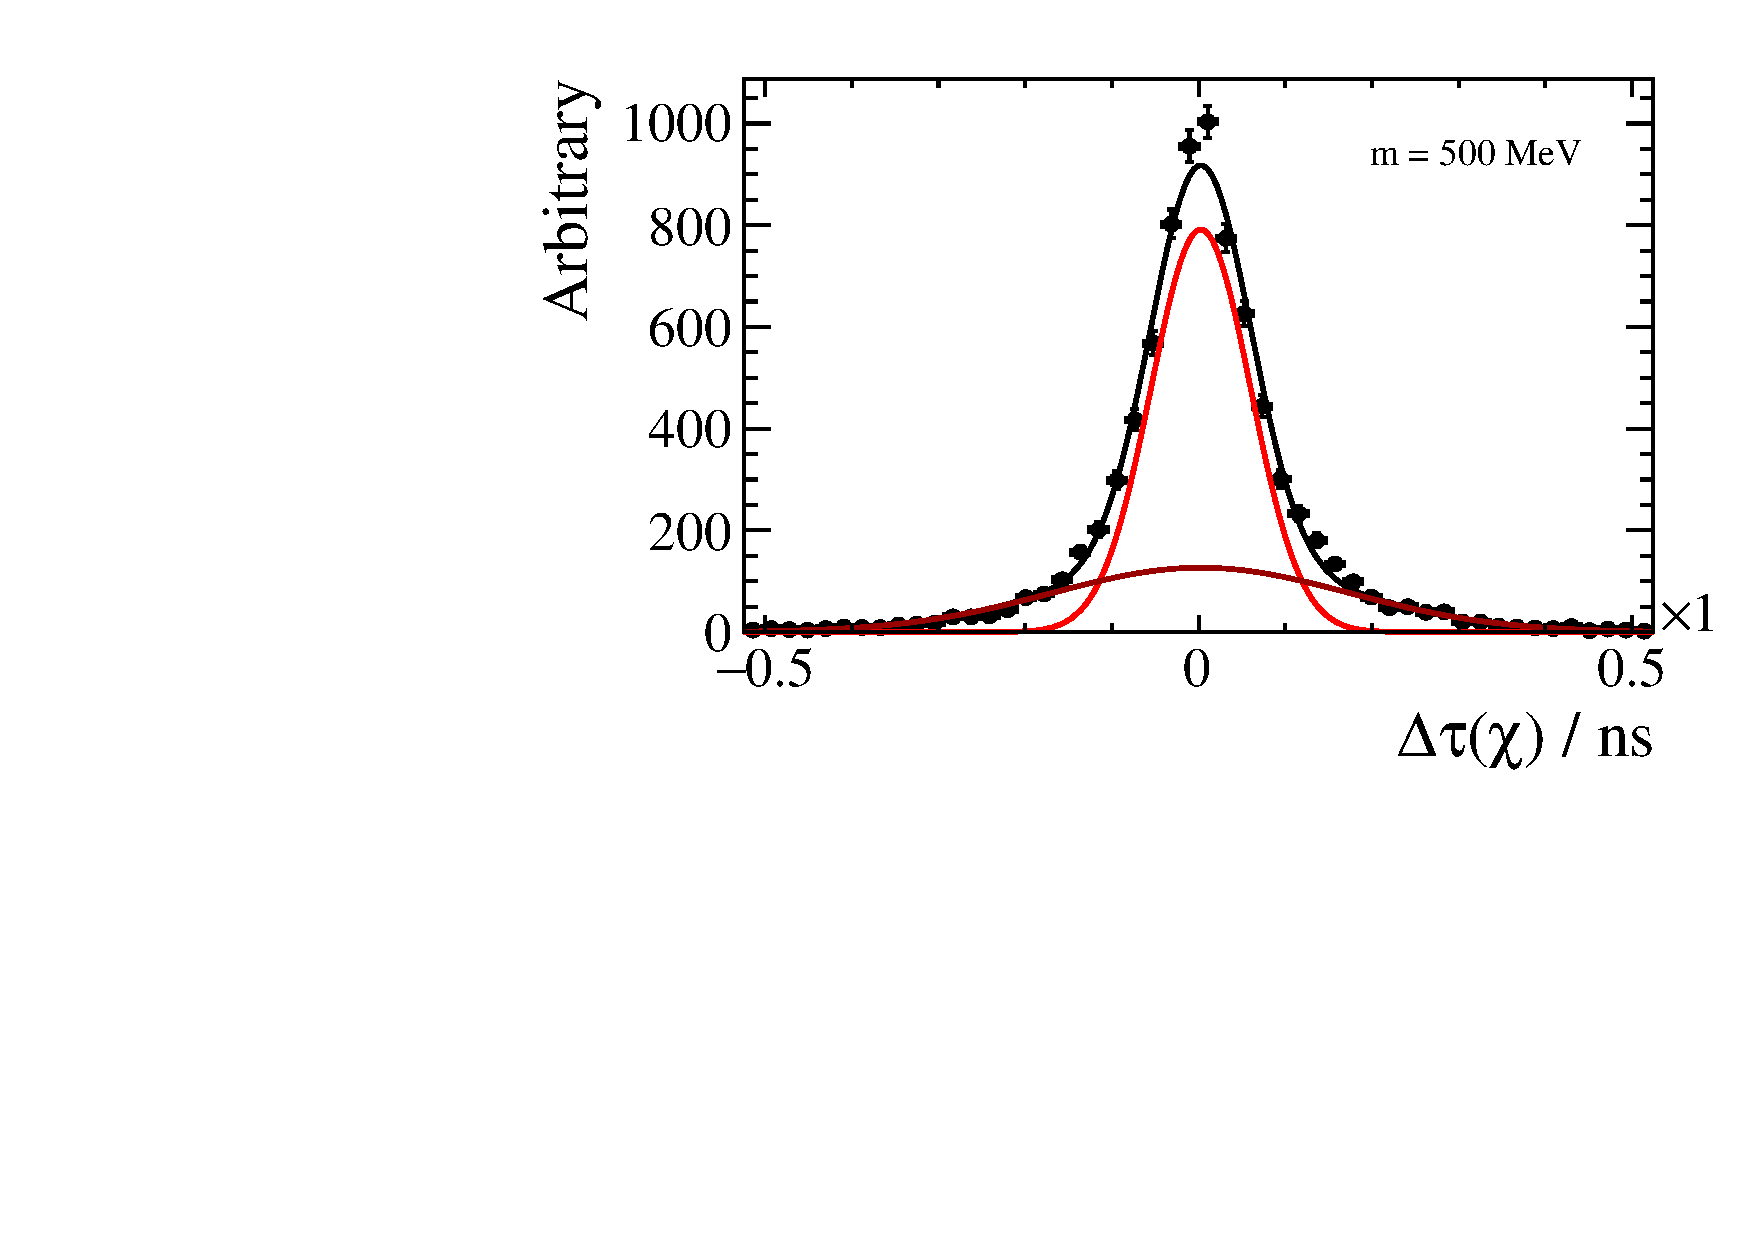
\includegraphics[width=0.42\textwidth]{anaTauResZoom_500}
    %%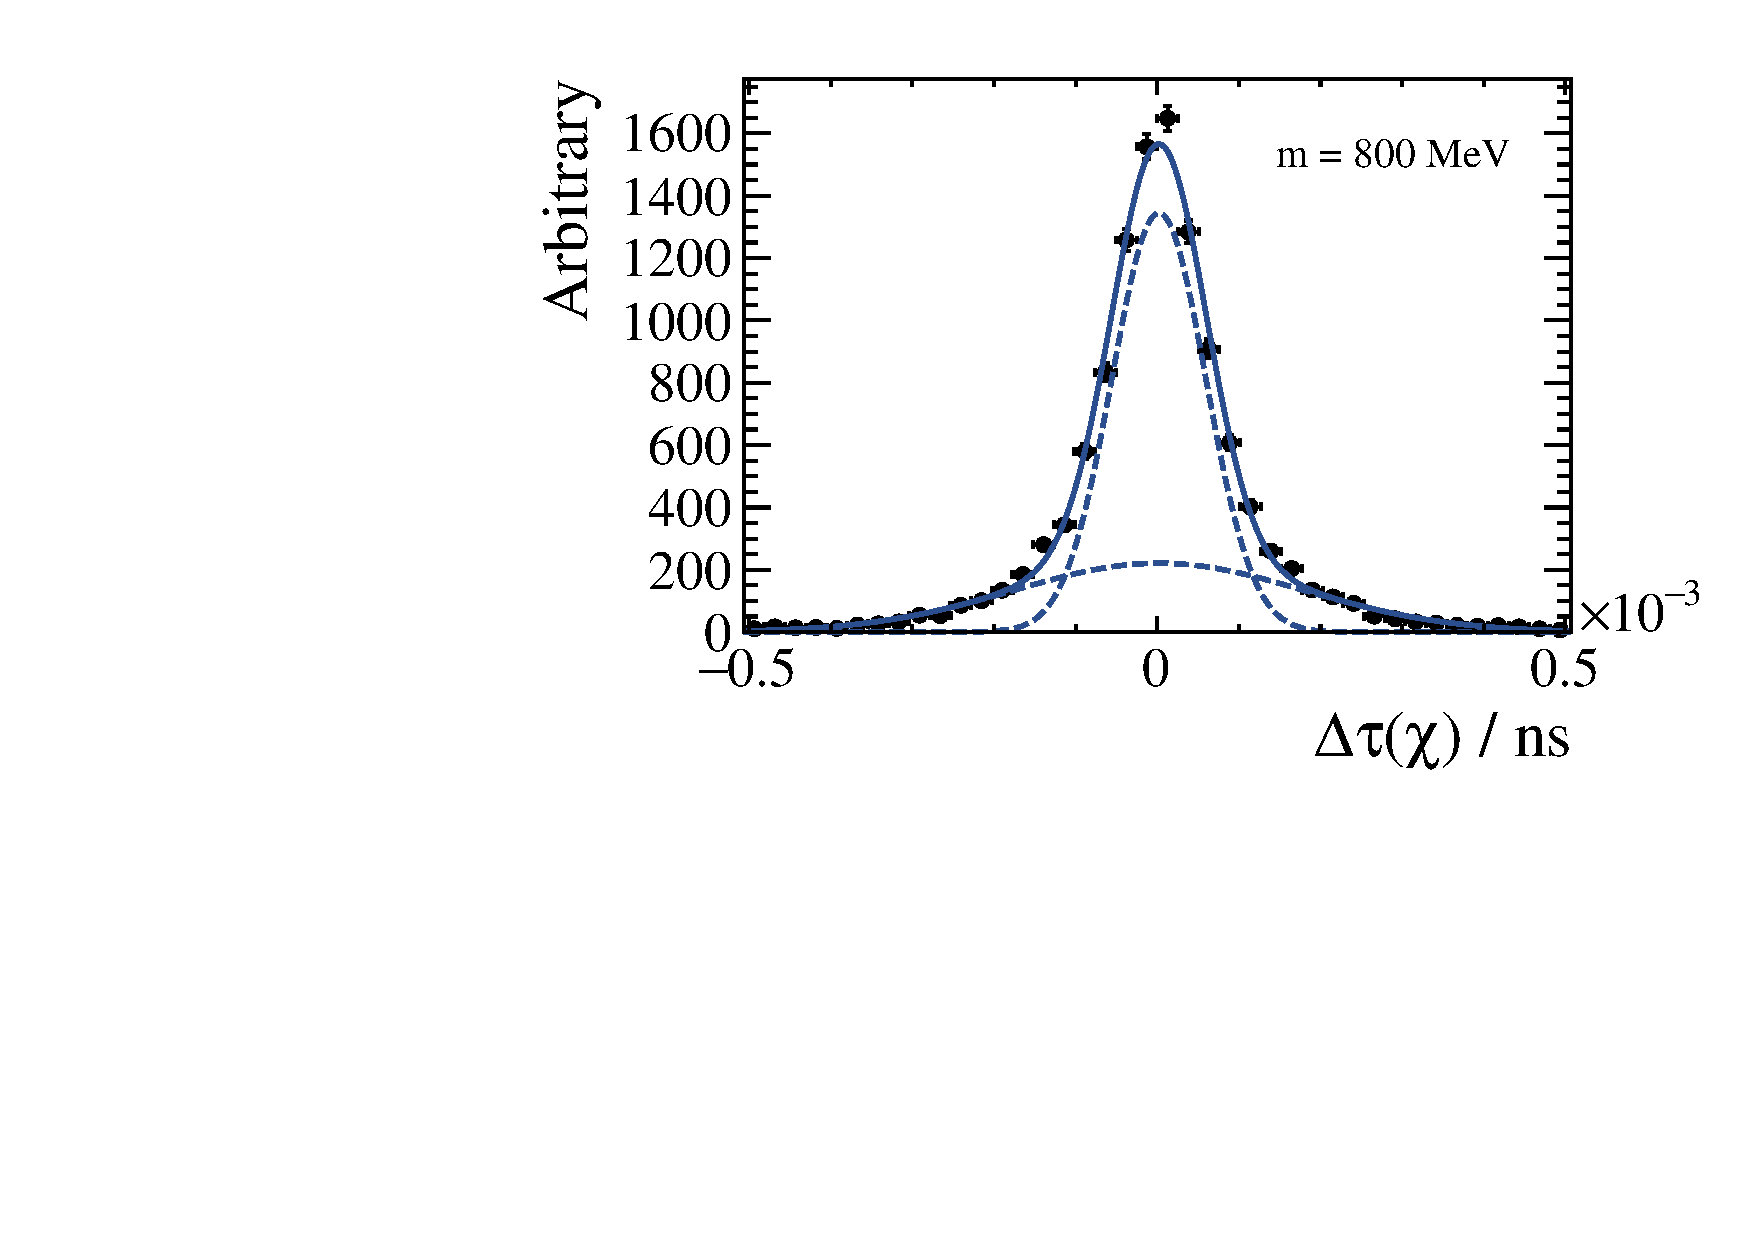
\includegraphics[width=0.42\textwidth]{anaTauResZoom_800}
    %%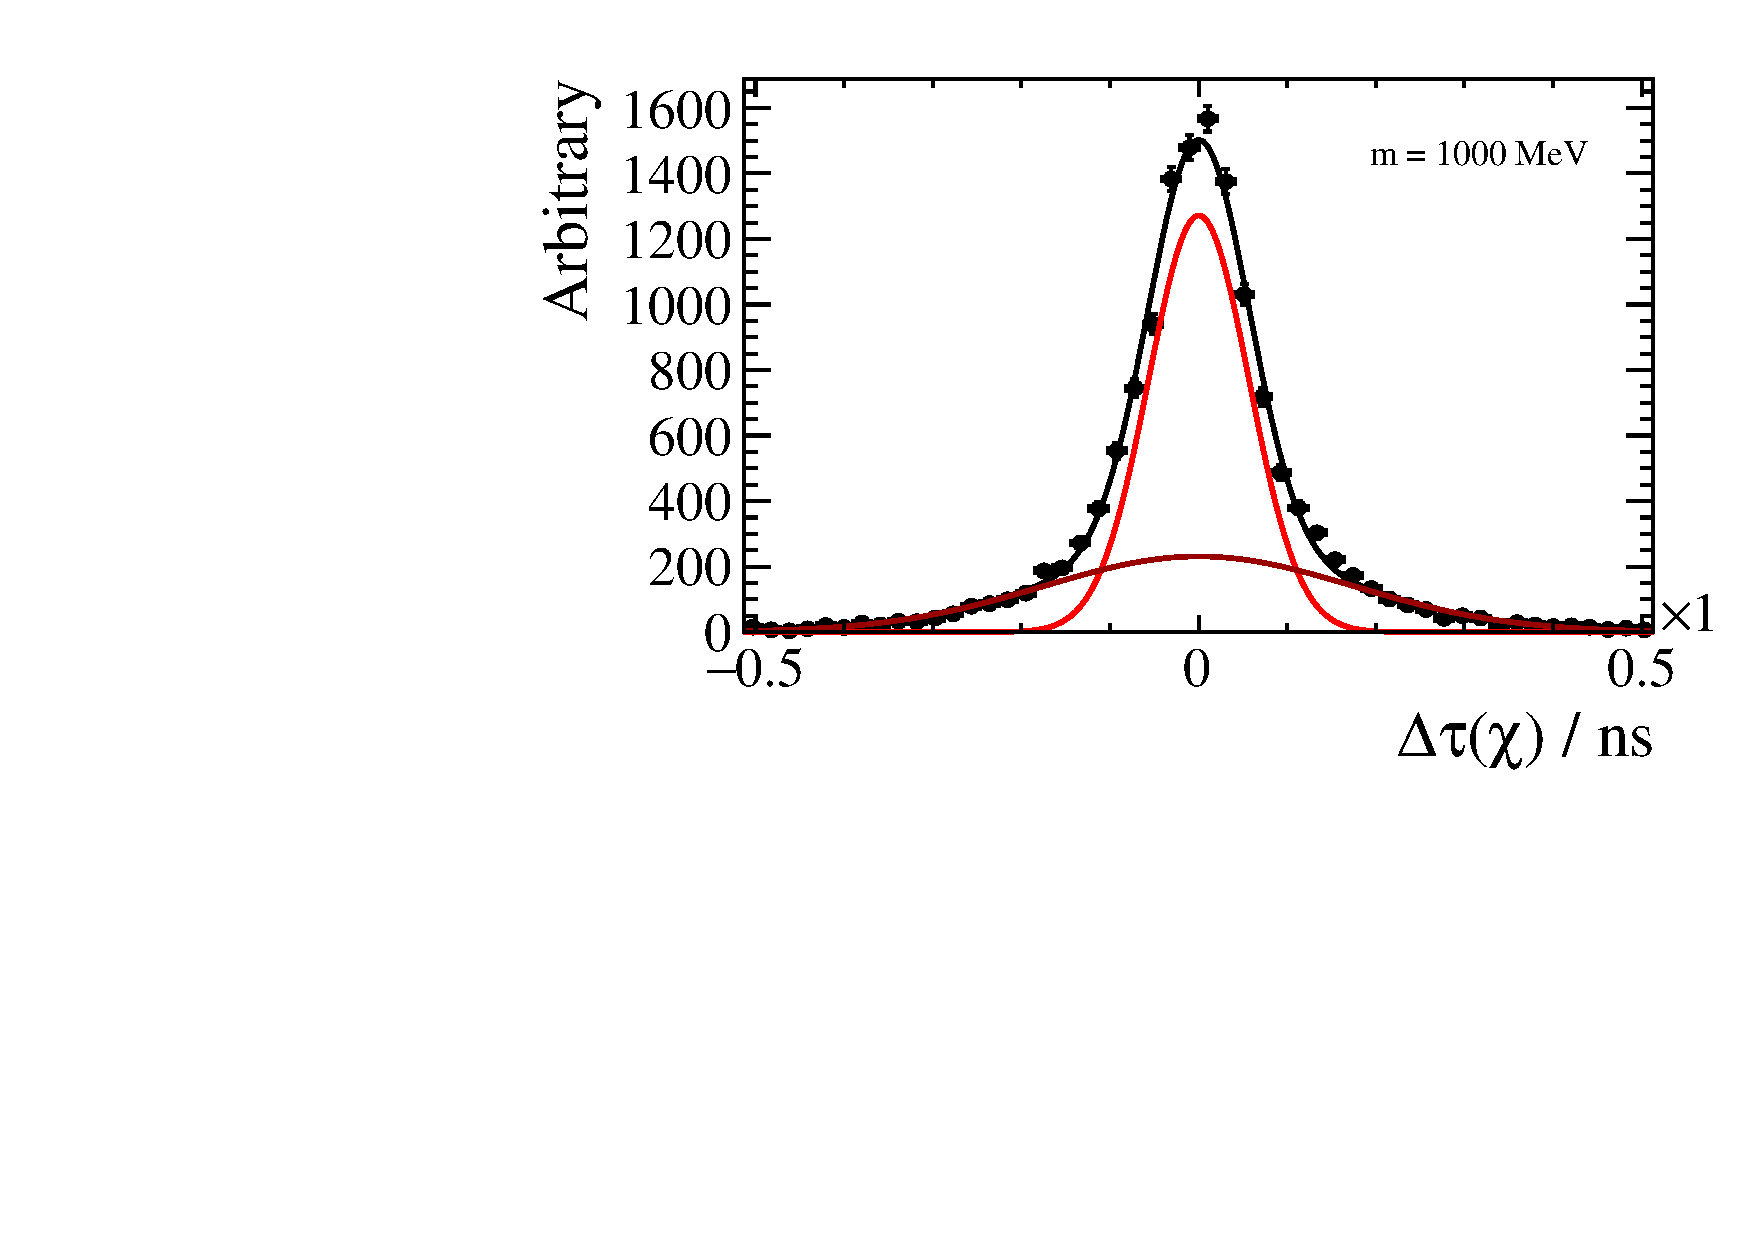
\includegraphics[width=0.42\textwidth]{anaTauResZoom_1000}
    %%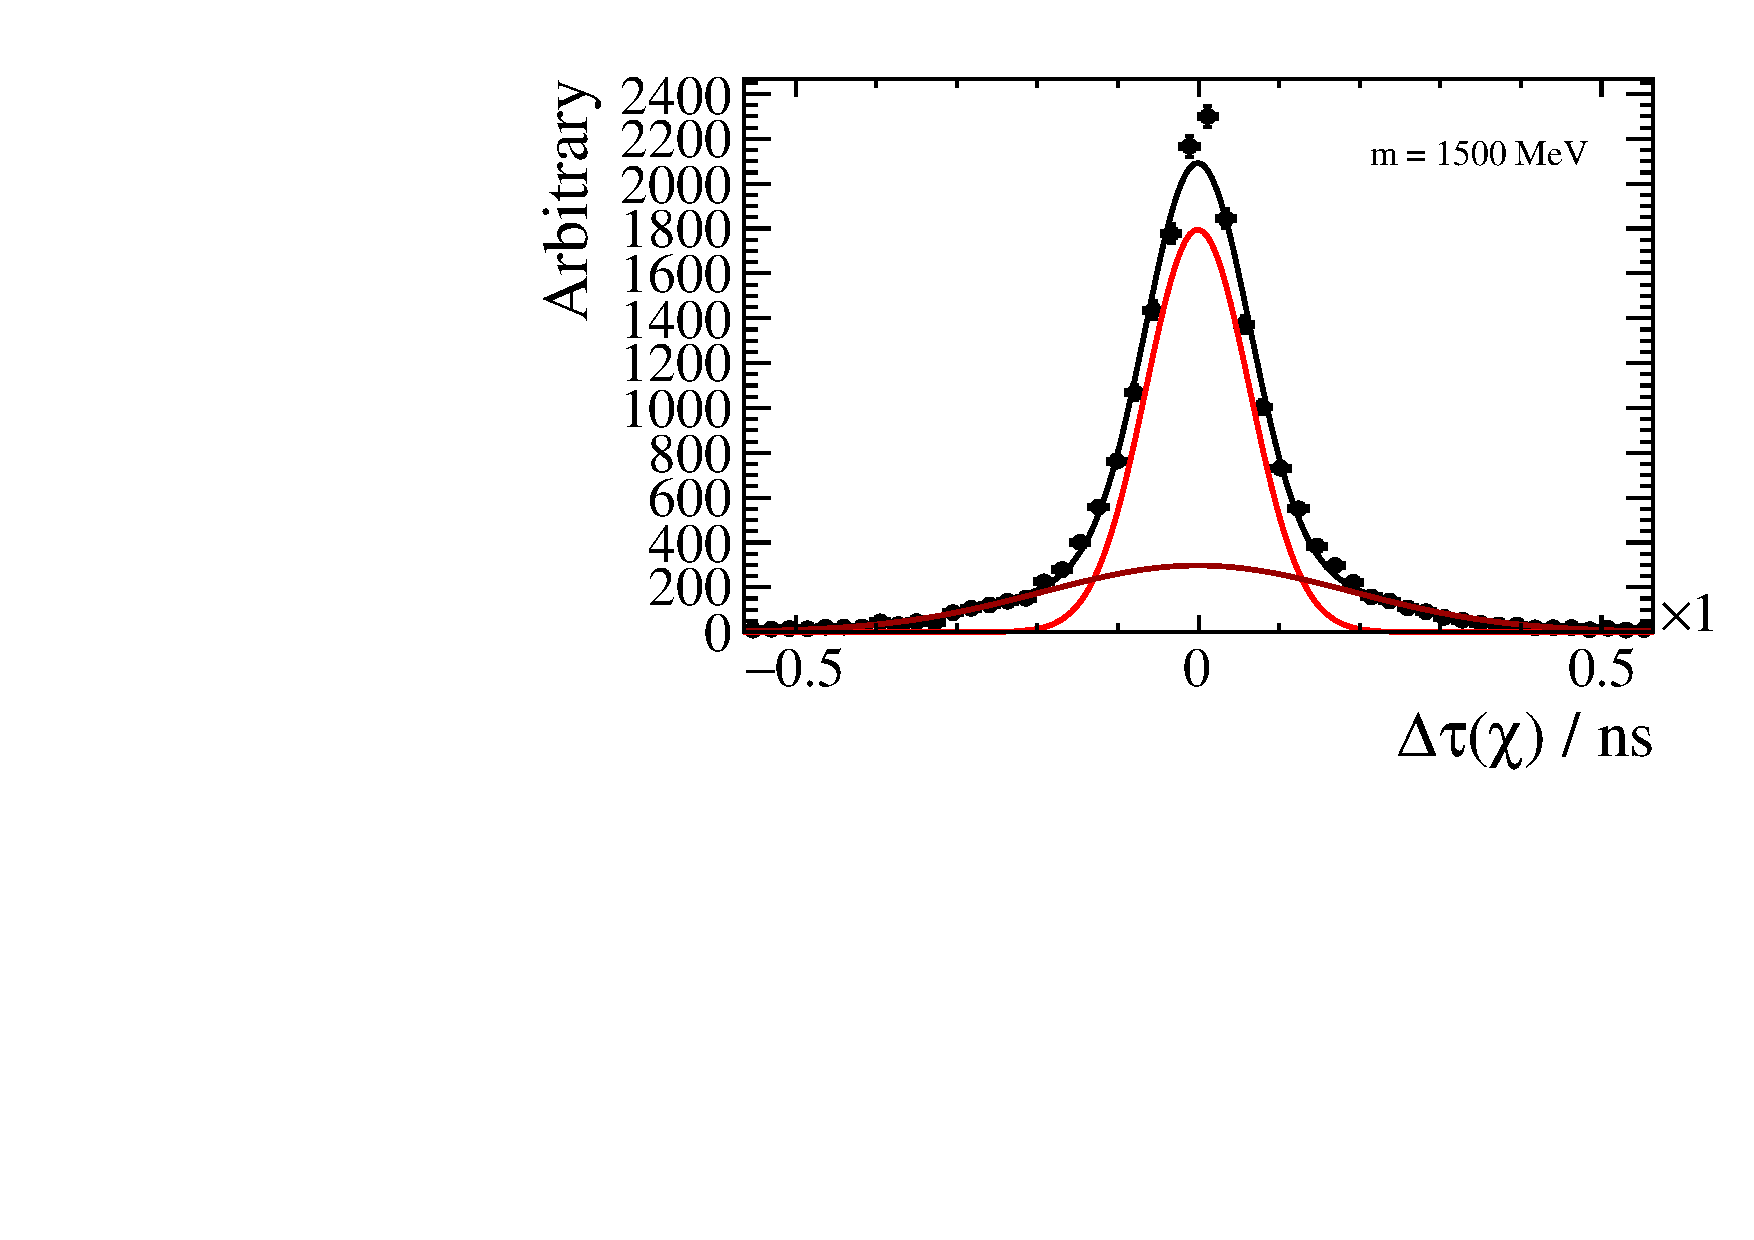
\includegraphics[width=0.42\textwidth]{anaTauResZoom_1500}
    %%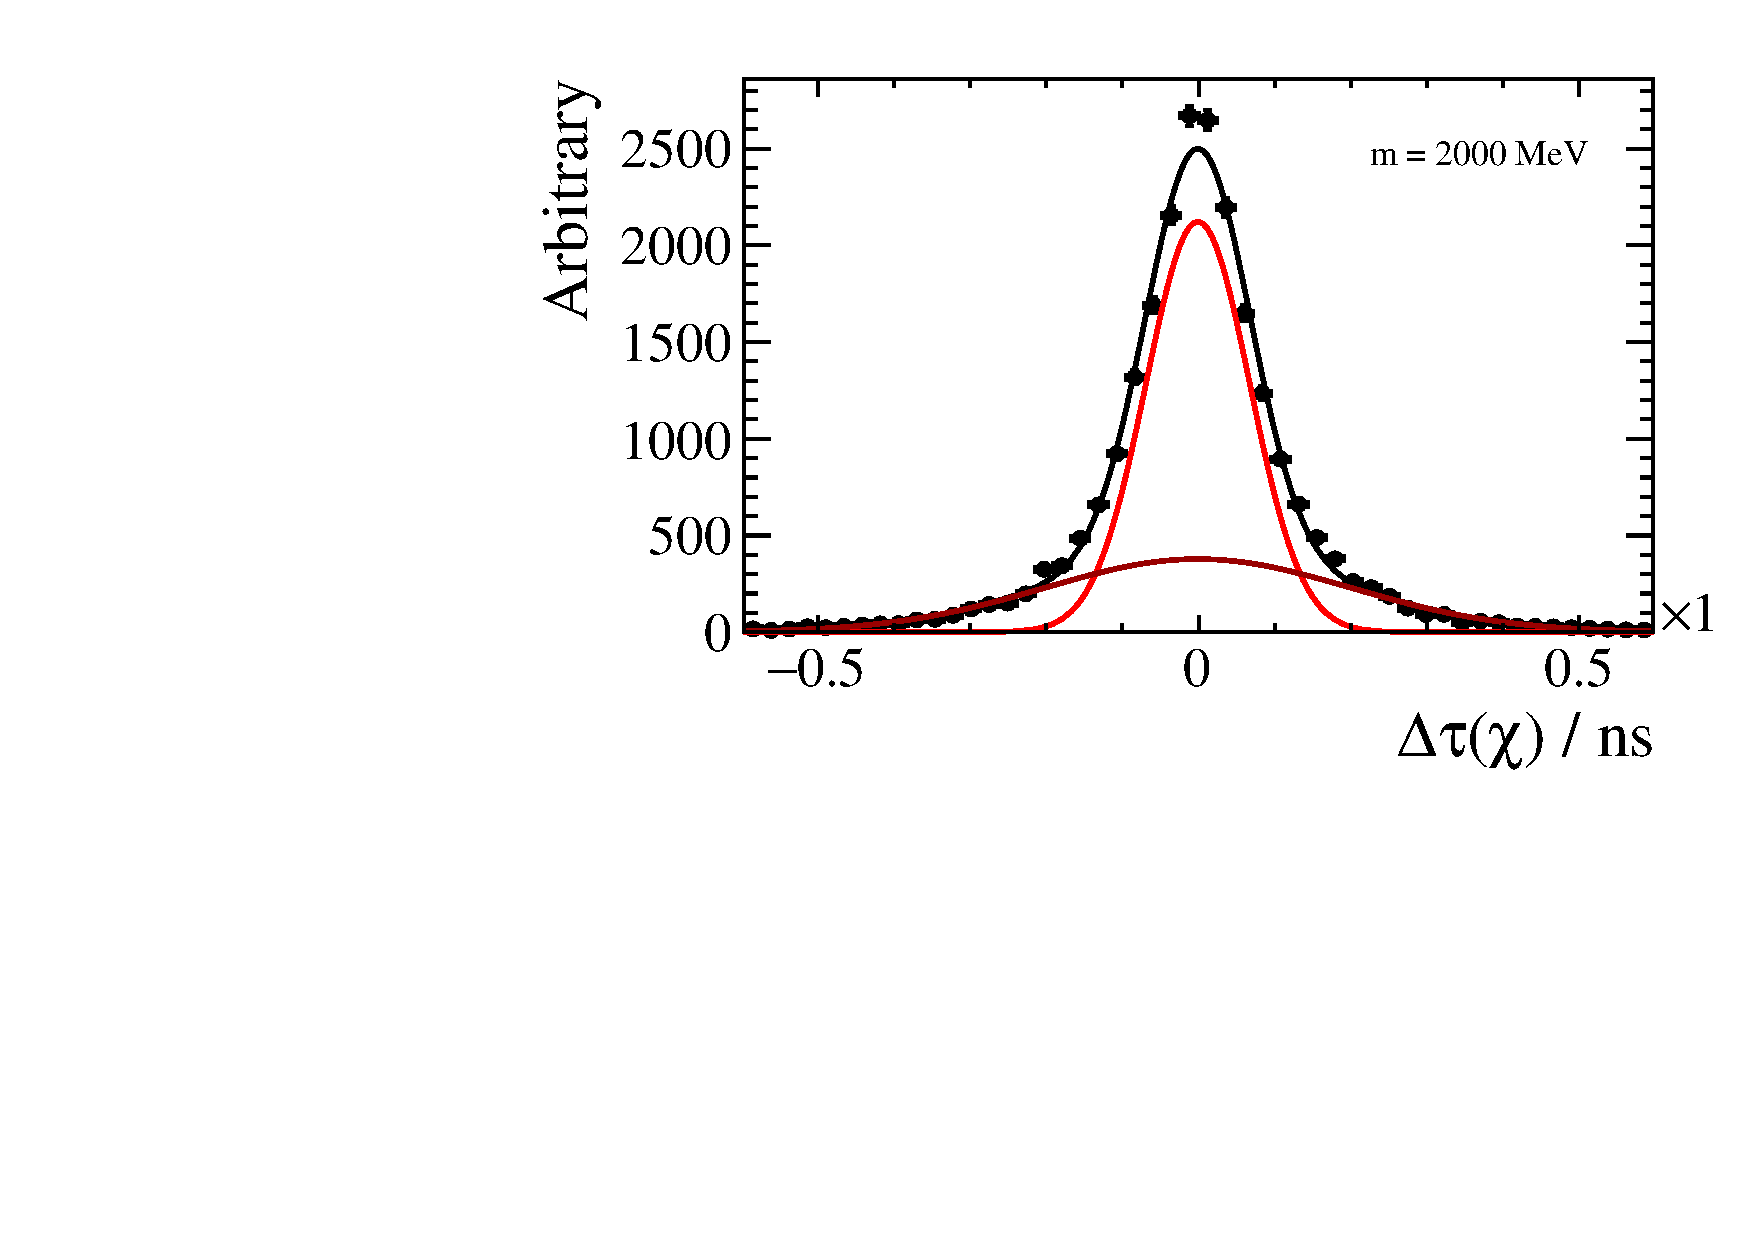
\includegraphics[width=0.42\textwidth]{anaTauResZoom_2000}
    %%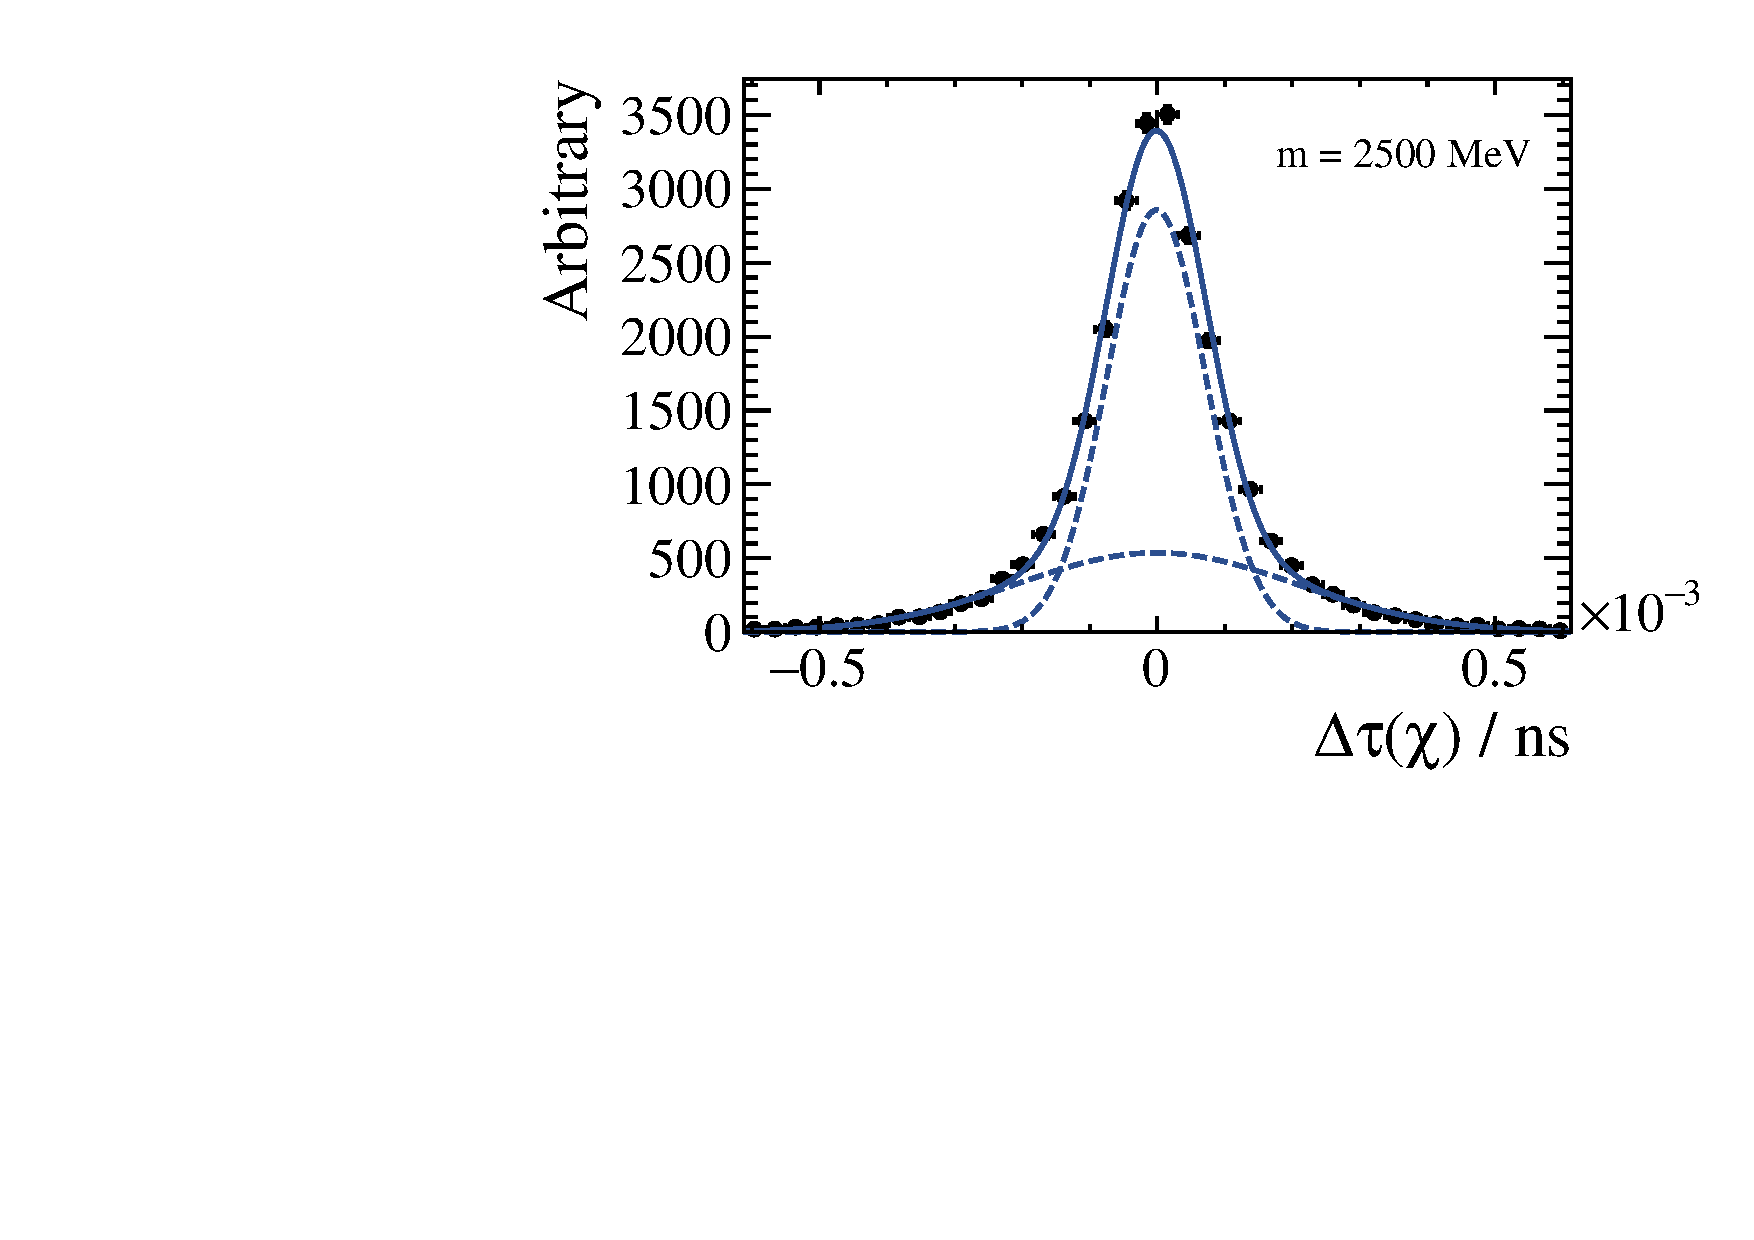
\includegraphics[width=0.42\textwidth]{anaTauResZoom_2500}
    %%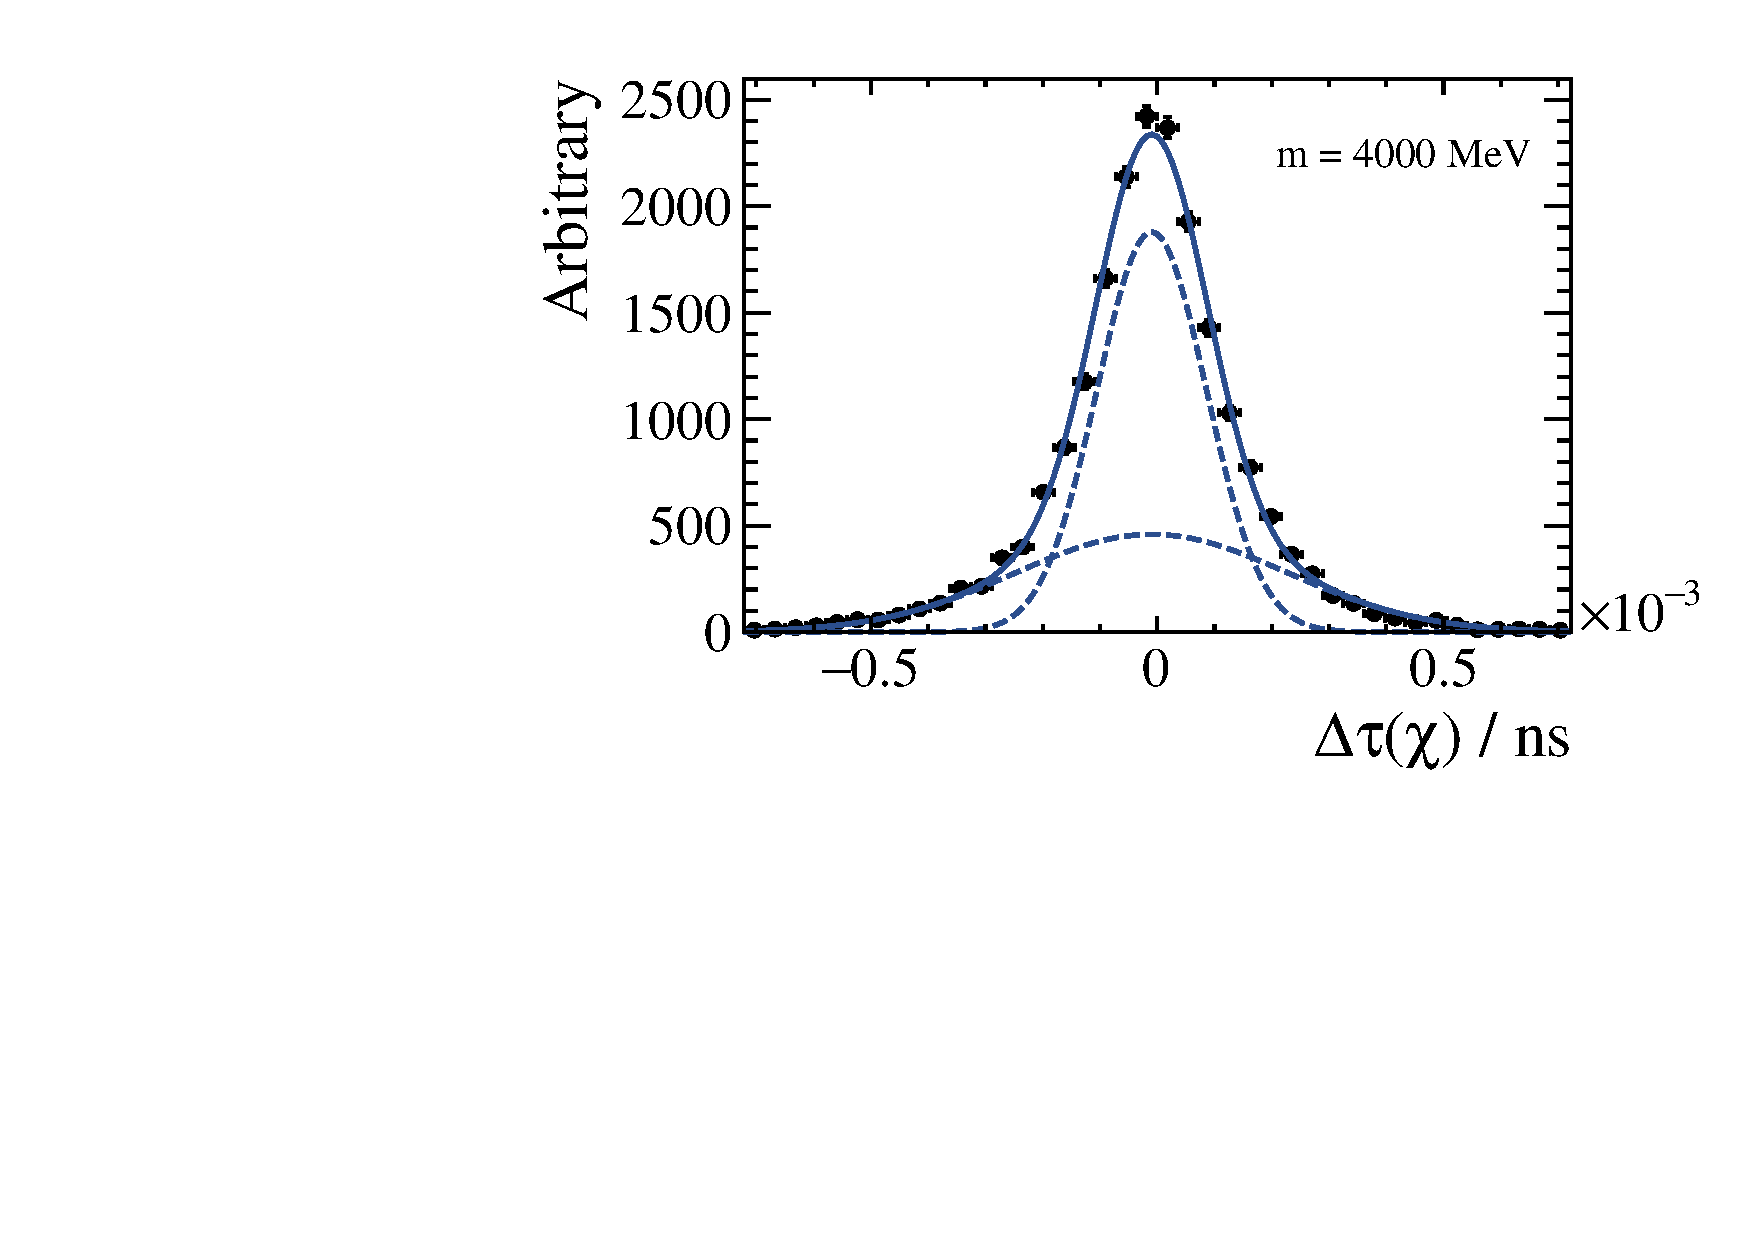
\includegraphics[width=0.42\textwidth]{anaTauResZoom_4000}
    %\includegraphics[width=0.42\textwidth]{anaTauRes_214}
    %\includegraphics[width=0.42\textwidth]{anaTauRes_220}
    %\includegraphics[width=0.42\textwidth]{anaTauRes_235}
    %\includegraphics[width=0.42\textwidth]{anaTauRes_250}
    %\includegraphics[width=0.42\textwidth]{anaTauRes_500}
    %%\includegraphics[width=0.42\textwidth]{anaTauRes_800}
    %\includegraphics[width=0.42\textwidth]{anaTauRes_1000}
    %%\includegraphics[width=0.42\textwidth]{anaTauRes_1500}
    %%\includegraphics[width=0.42\textwidth]{anaTauRes_2000}
    %\includegraphics[width=0.42\textwidth]{anaTauRes_2500}
    %\includegraphics[width=0.42\textwidth]{anaTauRes_4000}
  %\end{center}
  %\caption{\small
    %Fits to the lifetime resolution parameter, $\Delta\tau$, for individual mass samples.
    %Each fit for $m\geq250\mev$ is made using a double Gaussian function, and for $m<250\mev$ the
    %wider Gaussian has an exponential tail on the right-hand side.
  %}
  %\label{fig:taures:zoom}
%\end{figure}

%The source of the poor mass resolution at low mass is the \mumu opening angle, which is small near the dimuon mass threshold.
%This results in the separation of the hits in the first \velo station of the $\mu^+$ and $\mu^-$ being comparable to the resolution of the \velo strips which results in poor spatial resolution on the SV position.
%Furthermore, the hits are often merged in the \velo, producing a reconstructed SV position downstream of the true position.
%From the distributions of reconstructed and generated opening angles for $m=214\mev$ in Fig.~\ref{fig:opening:gen},
%it can be seen that there is no bias once the \mumu opening angle exceeds $\sim0.002$ radians.
%Vetoing all events below this threshold is a very inefficient solution at low dimuon
%masses, (see Fig.~\ref{fig:opening:gen}).
%Instead, the bias is accounted for, as described below.

%%The observation of the discrepancy between real and true opening angle will be verified using data
%%from a decay channel with very high statistics.
%%The decay \decay{\Bs}{\jpsi\kk} should show the same thing for low \kk mass.


%\begin{figure}
  %\begin{center}
    %\subfloat[\label{fig:oa:214}]{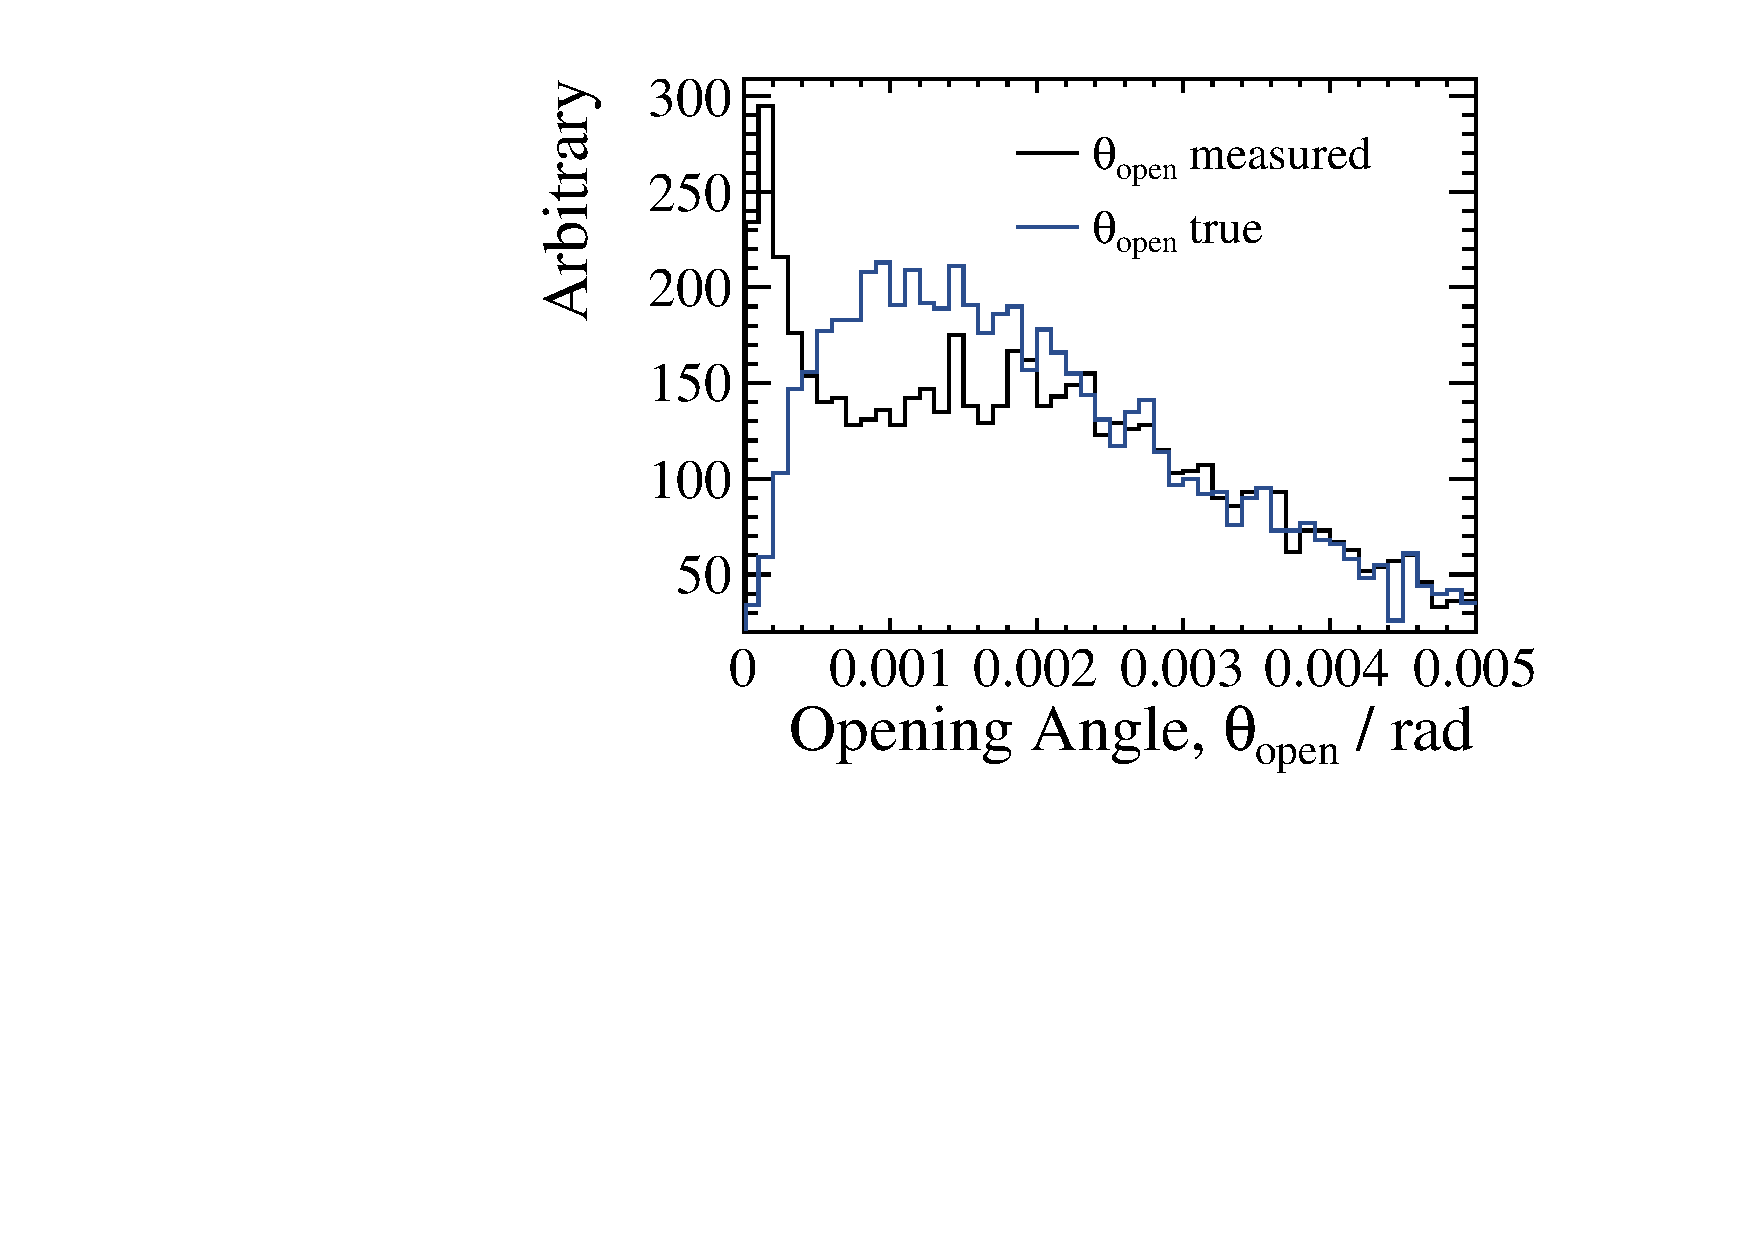
\includegraphics[width=0.48\textwidth]{ana214Opening}}
    %\subfloat[\label{fig:oa:gen}]{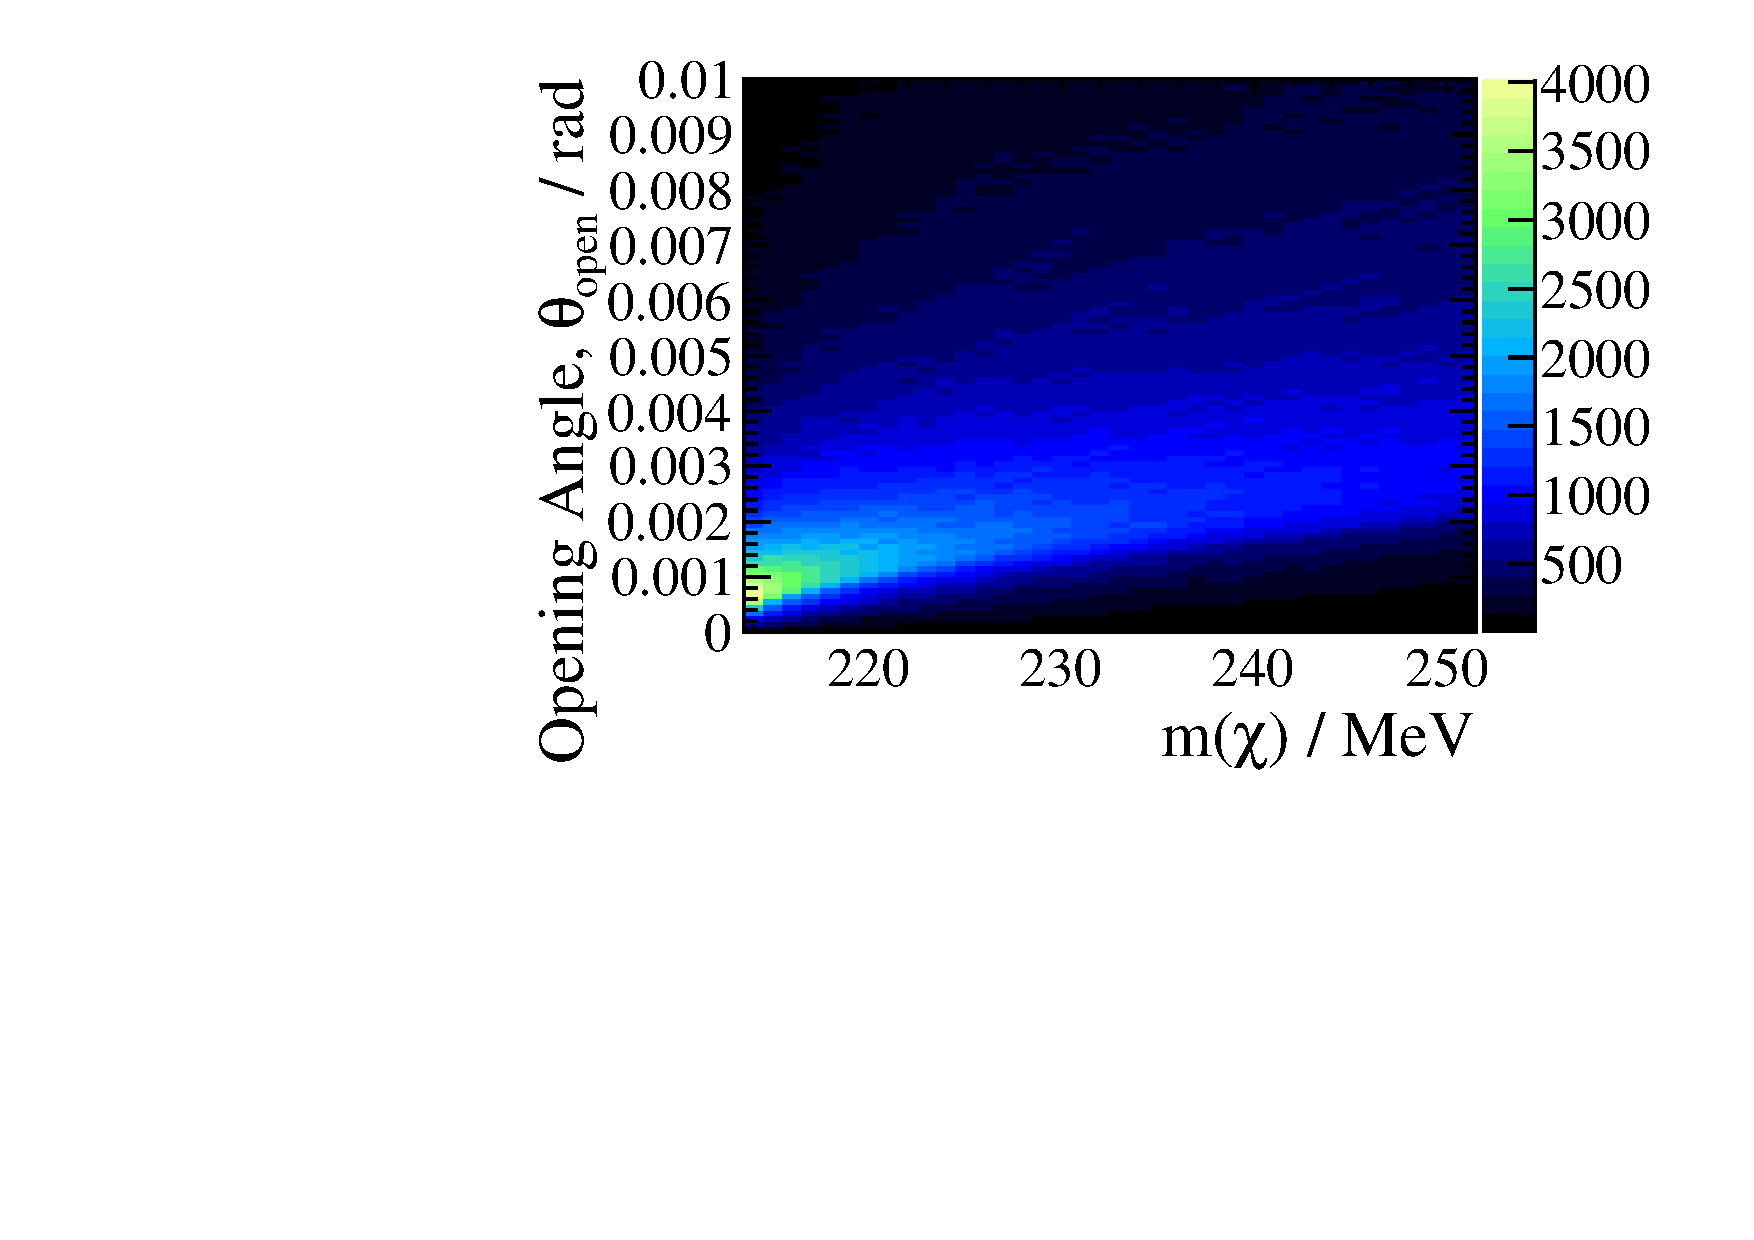
\includegraphics[width=0.48\textwidth]{anaGenLevelOpening}}
  %\end{center}
  %\caption{\small
    %The opening angle of the two muons decaying from the \db is highly dependent on \mdb; for low
    %dimuon masses the opening angle measurement is biased.
    %For $\mdb=214\mev$ the difference between generated and reconstructed opening angles are shown,
    %\protect\subref{fig:oa:214}, the greatest difference being below $\theta_\mathrm{open}=0.002$.
    %Generator level distributions of opening angles for a range of masses,
    %\protect\subref{fig:oa:gen}, show that most \db decays have $\theta_\mathrm{open}>0.002$ for
    %$\mdb\gtrsim235\mev$.
  %}
  %\label{fig:opening:gen}
%\end{figure}

%The observation of the discrepancy between real and true opening angle can be verified using data
%from a decay channel with very high statistics, for example,
%the decay \decay{\Bd}{\kpi\mumu}, where the muons can come from any resonance.
%Figure~\ref{fig:oa:2d} shows how the opening angle of the \kpi system changes with its invariant
%mass (for $m_{\kpi}<900\mev$); it is seen that at threshold, the opening angle is observed to be
%very small for low masses, especially at threshold, $m_{\Kp} + m_{\pim} = 633.3\mev$.
%A one dimensional plot of the opening angle for $m_{\kpi}<640\mev$ is shown in \Fig{fig:oa:1d}.
%It is seen that the \kpi opening angle at low mass does indeed have a peak at $\sim\!0$, as
%observed in the simulation in \Fig{fig:oa}

%\begin{figure}
  %\begin{center}
    %\subfloat[\label{fig:oa:2d}]{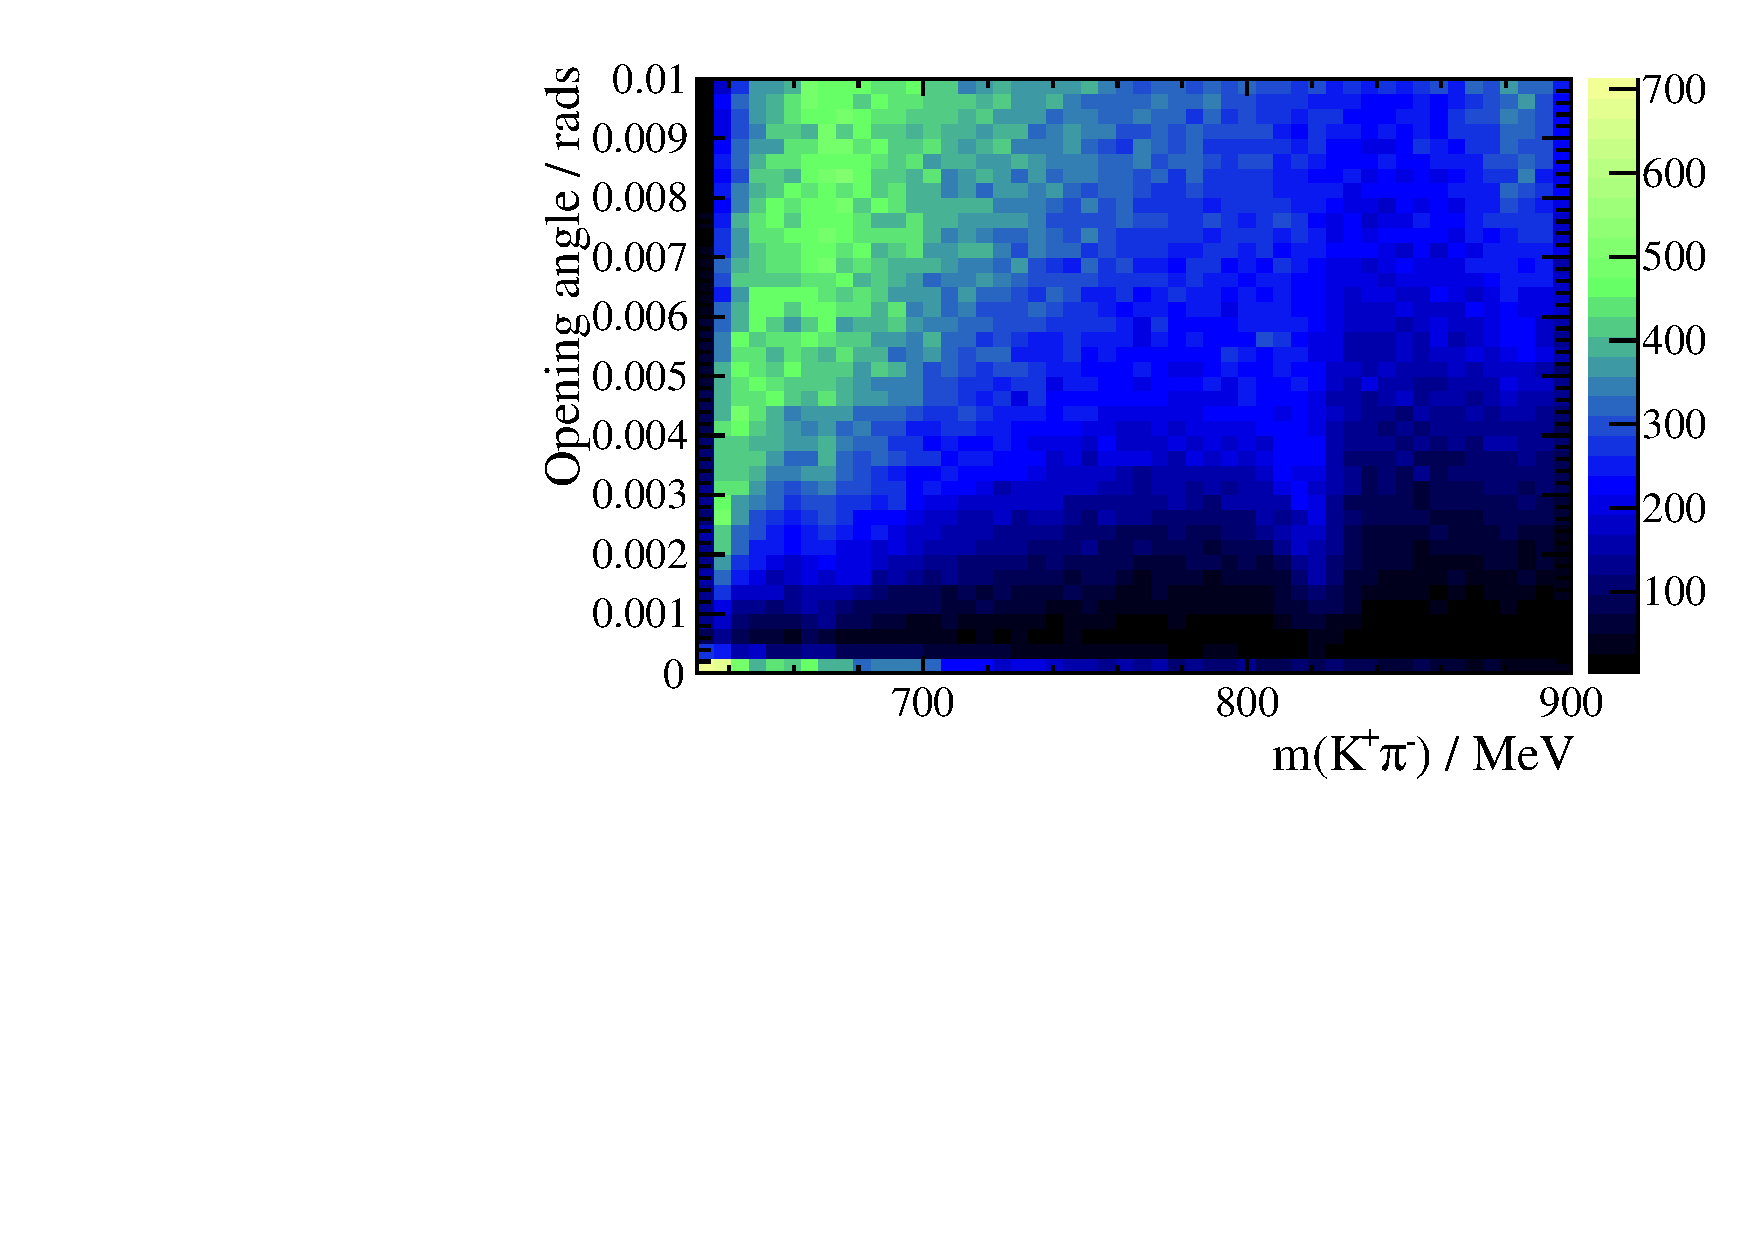
\includegraphics[width=0.48\textwidth]{opening_angle_data_2d}}
    %\subfloat[\label{fig:oa:1d}]{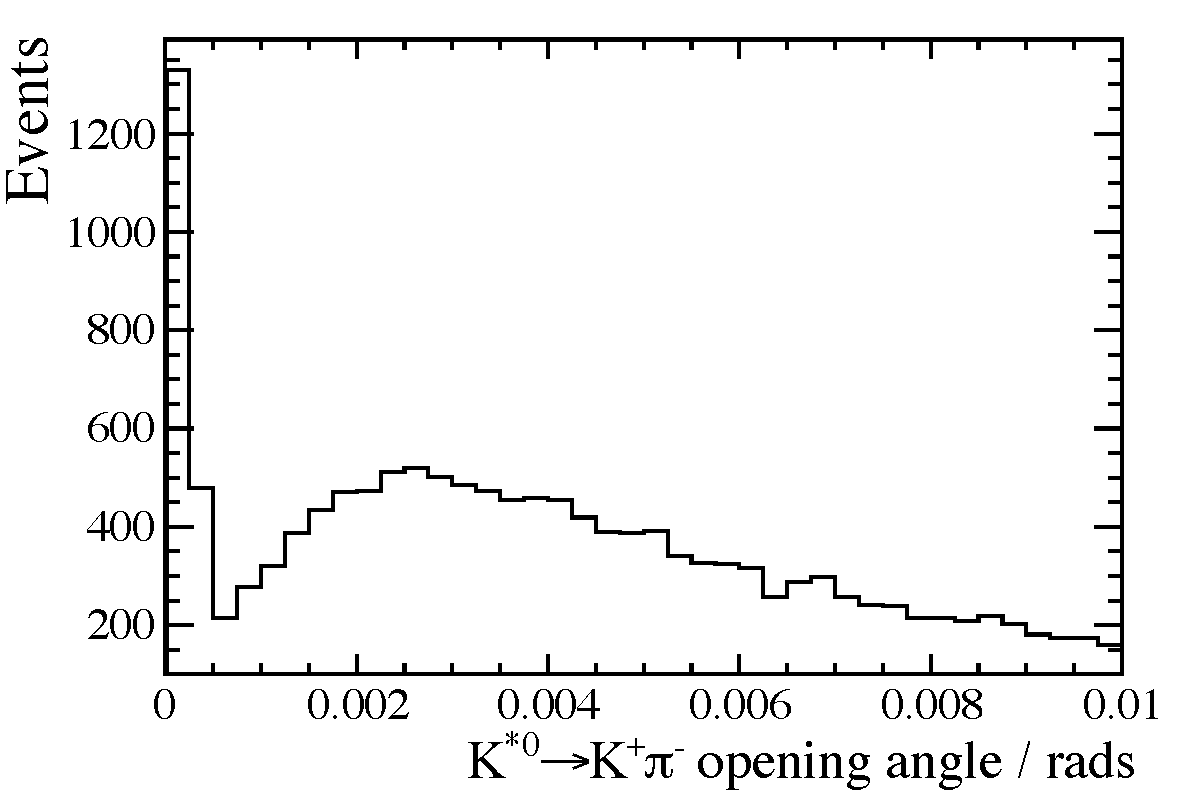
\includegraphics[width=0.48\textwidth]{opening_angle_data}}
    %\caption{\small
      %Opening angles of the \kpi system in the decay \decay{\Bd}{\kpi\mumu}, where there is no mass
      %constraint on the muons.
      %A two dimensional plot of $m_{\kpi}$ against opening angle is shown in
      %Fig.~\protect\subref{fig:oa:2d}, where there is a peak for an opening angle of $\sim\!0$ for
      %low $m_{\kpi}$, which becomes much less significant as the mass of the \kpi system grows.
      %Figure~\protect\subref{fig:oa:1d} shows the slice in opening angle for $m_{\kpi}<640\mev$.
    %}
    %\label{fig:oa}
  %\end{center}
%\end{figure}



%\begin{figure}
  %\begin{center}
    %\includegraphics[width=0.42\textwidth]{deltafd_214}
    %\includegraphics[width=0.42\textwidth]{deltafd_220}
    %\includegraphics[width=0.42\textwidth]{deltafd_235}
    %\includegraphics[width=0.42\textwidth]{deltafd_250}
    %\includegraphics[width=0.42\textwidth]{deltafd_500}
    %%\includegraphics[width=0.42\textwidth]{deltafd_800}
    %\includegraphics[width=0.42\textwidth]{deltafd_1000}
    %%\includegraphics[width=0.42\textwidth]{deltafd_1500}
    %%\includegraphics[width=0.42\textwidth]{deltafd_2000}
    %\includegraphics[width=0.42\textwidth]{deltafd_2500}
    %\includegraphics[width=0.42\textwidth]{deltafd_4000}
  %\end{center}
  %\caption{\small
    %Difference between the measured and true flight distances for a range of \db masses.
  %}
  %\label{fig:fd:zoom}
%\end{figure}

%The lifetime resolution is calculated at each mass point using a fit to $\Delta\tau$.
%Each PDF is constructed as the sum of two Gaussian functions.
%However, for the reasons described above, the low mass ($<250\mev$) has a tail extending to high
%lifetimes, and therefore for these samples an exponential tail is added to the Gaussian with larger width.
%These fits are shown in \Fig{fig:taures:zoom}; the same distributions for flight distance (without
%fits) are shown in \Fig{fig:fd:zoom}.
%The $3\,\sigma$ lifetime resolution is calculated from the fitted PDFs, which are
%shown in Fig.~\ref{fig:eff:spline:res}.

%\begin{figure}
  %\begin{center}
    %\subfloat[\label{fig:eff:spline:res}]{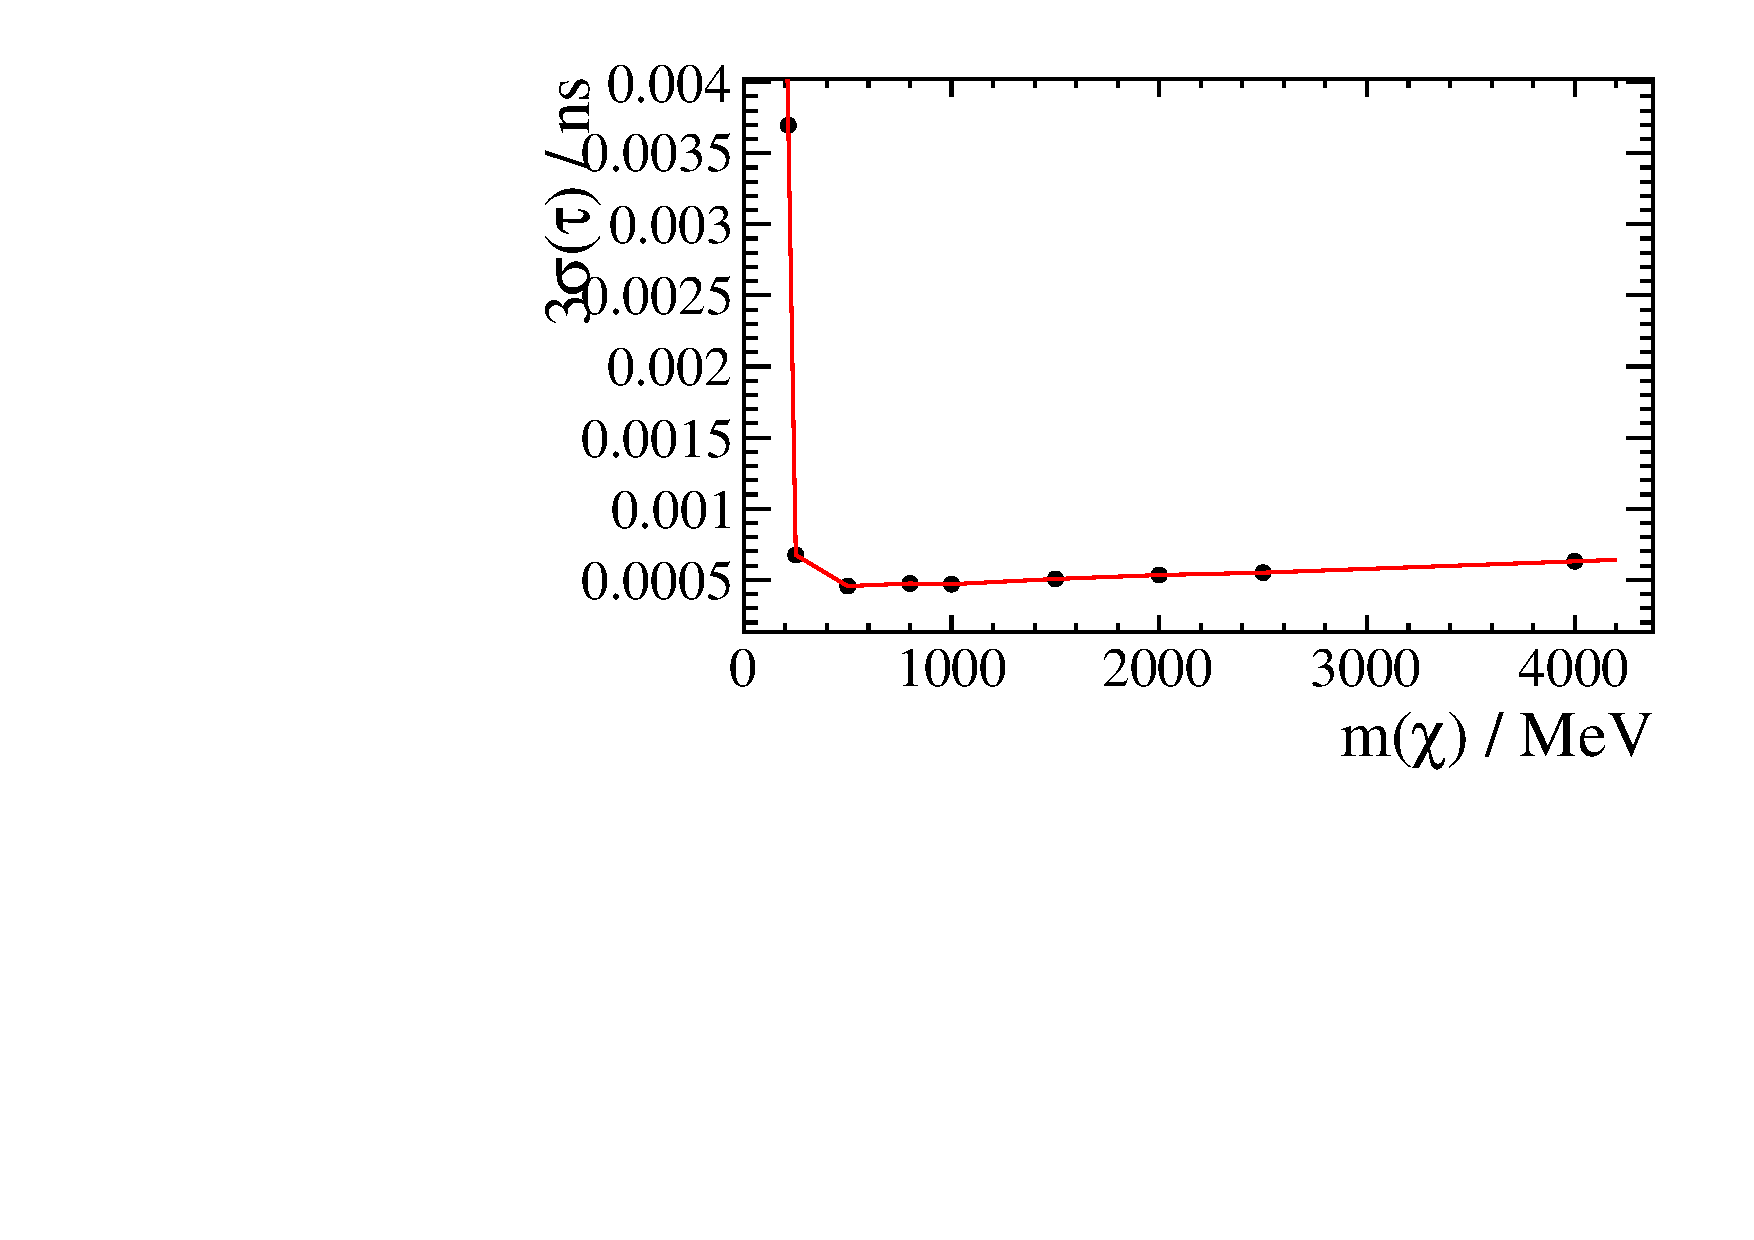
\includegraphics[width=0.48\textwidth]{spline_taures_upper}}
    %\subfloat[\label{fig:eff:spline:resl0}]{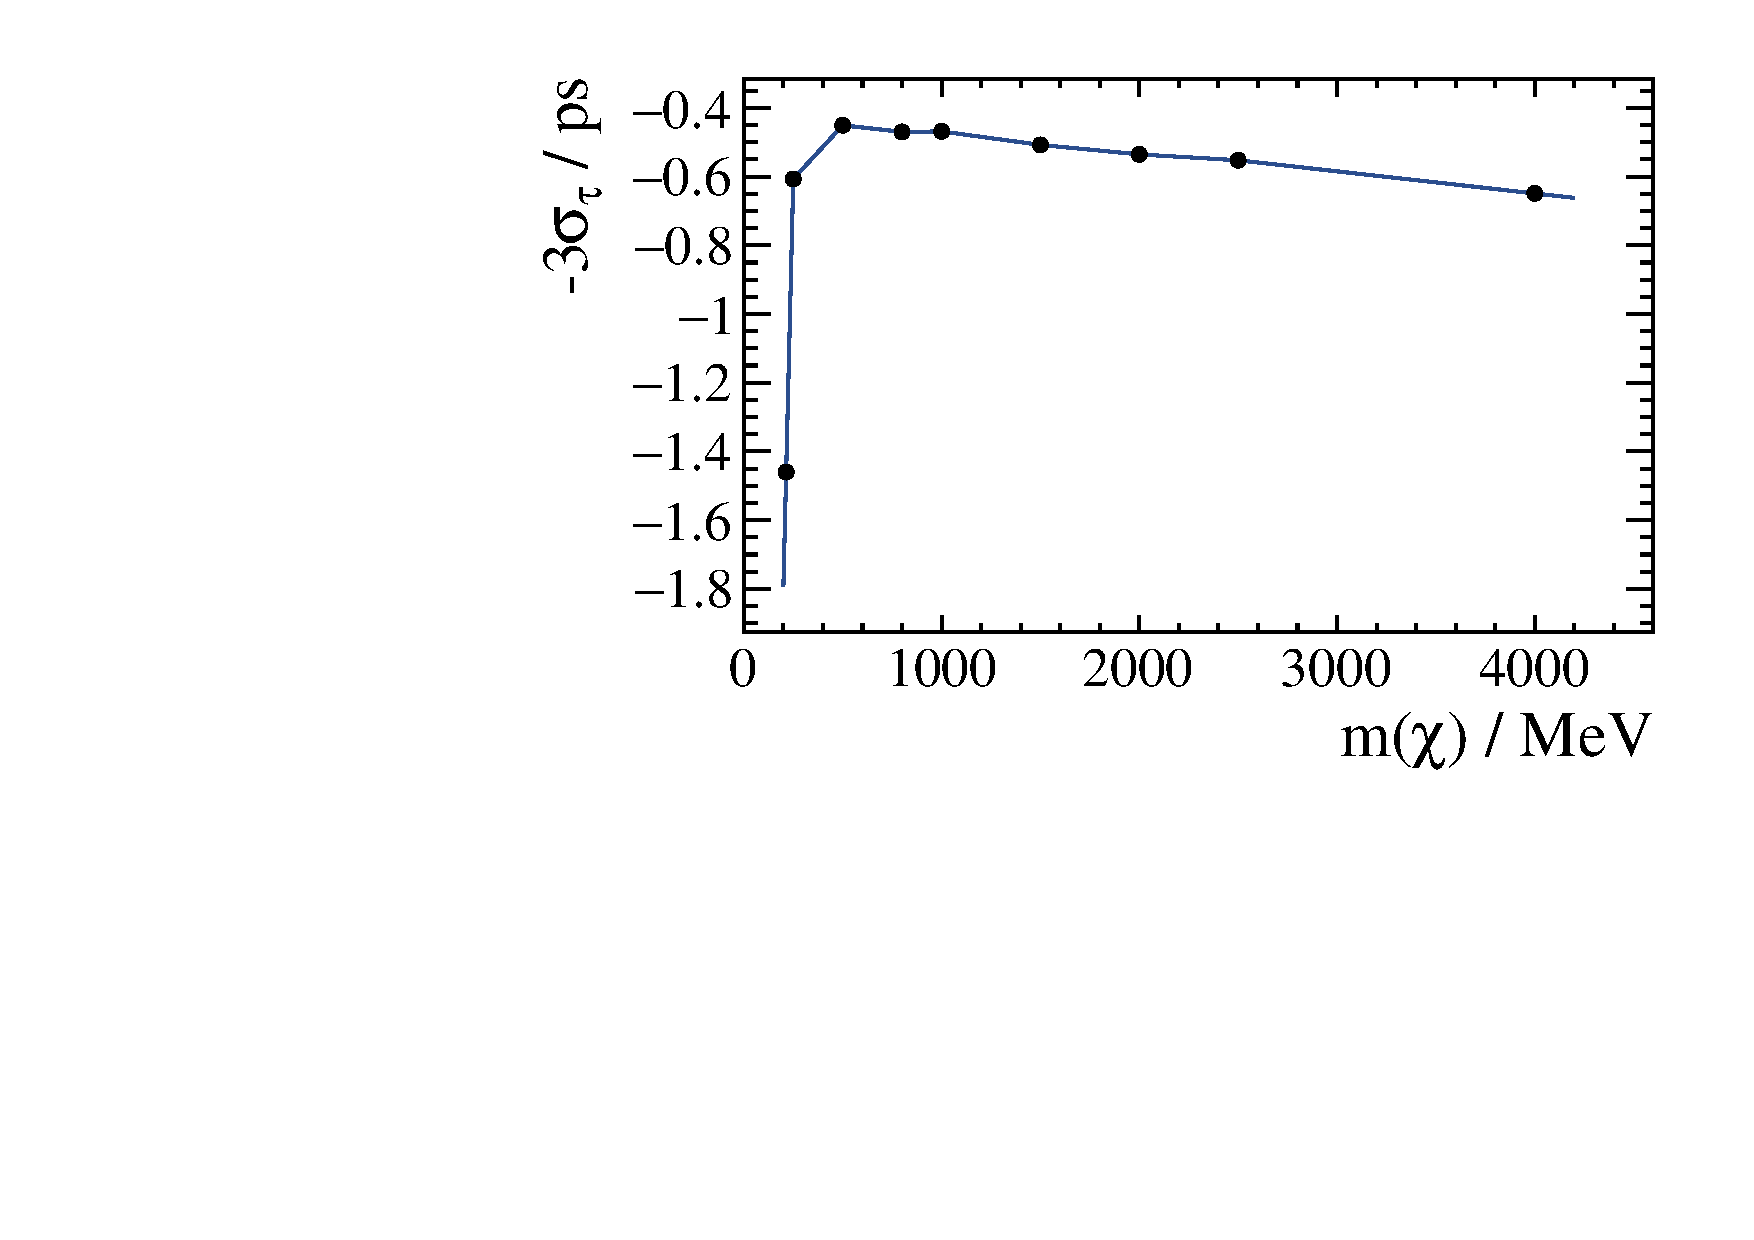
\includegraphics[width=0.48\textwidth]{spline_taures_lower}}\\
    %\subfloat[\label{fig:eff:spline:mass}]{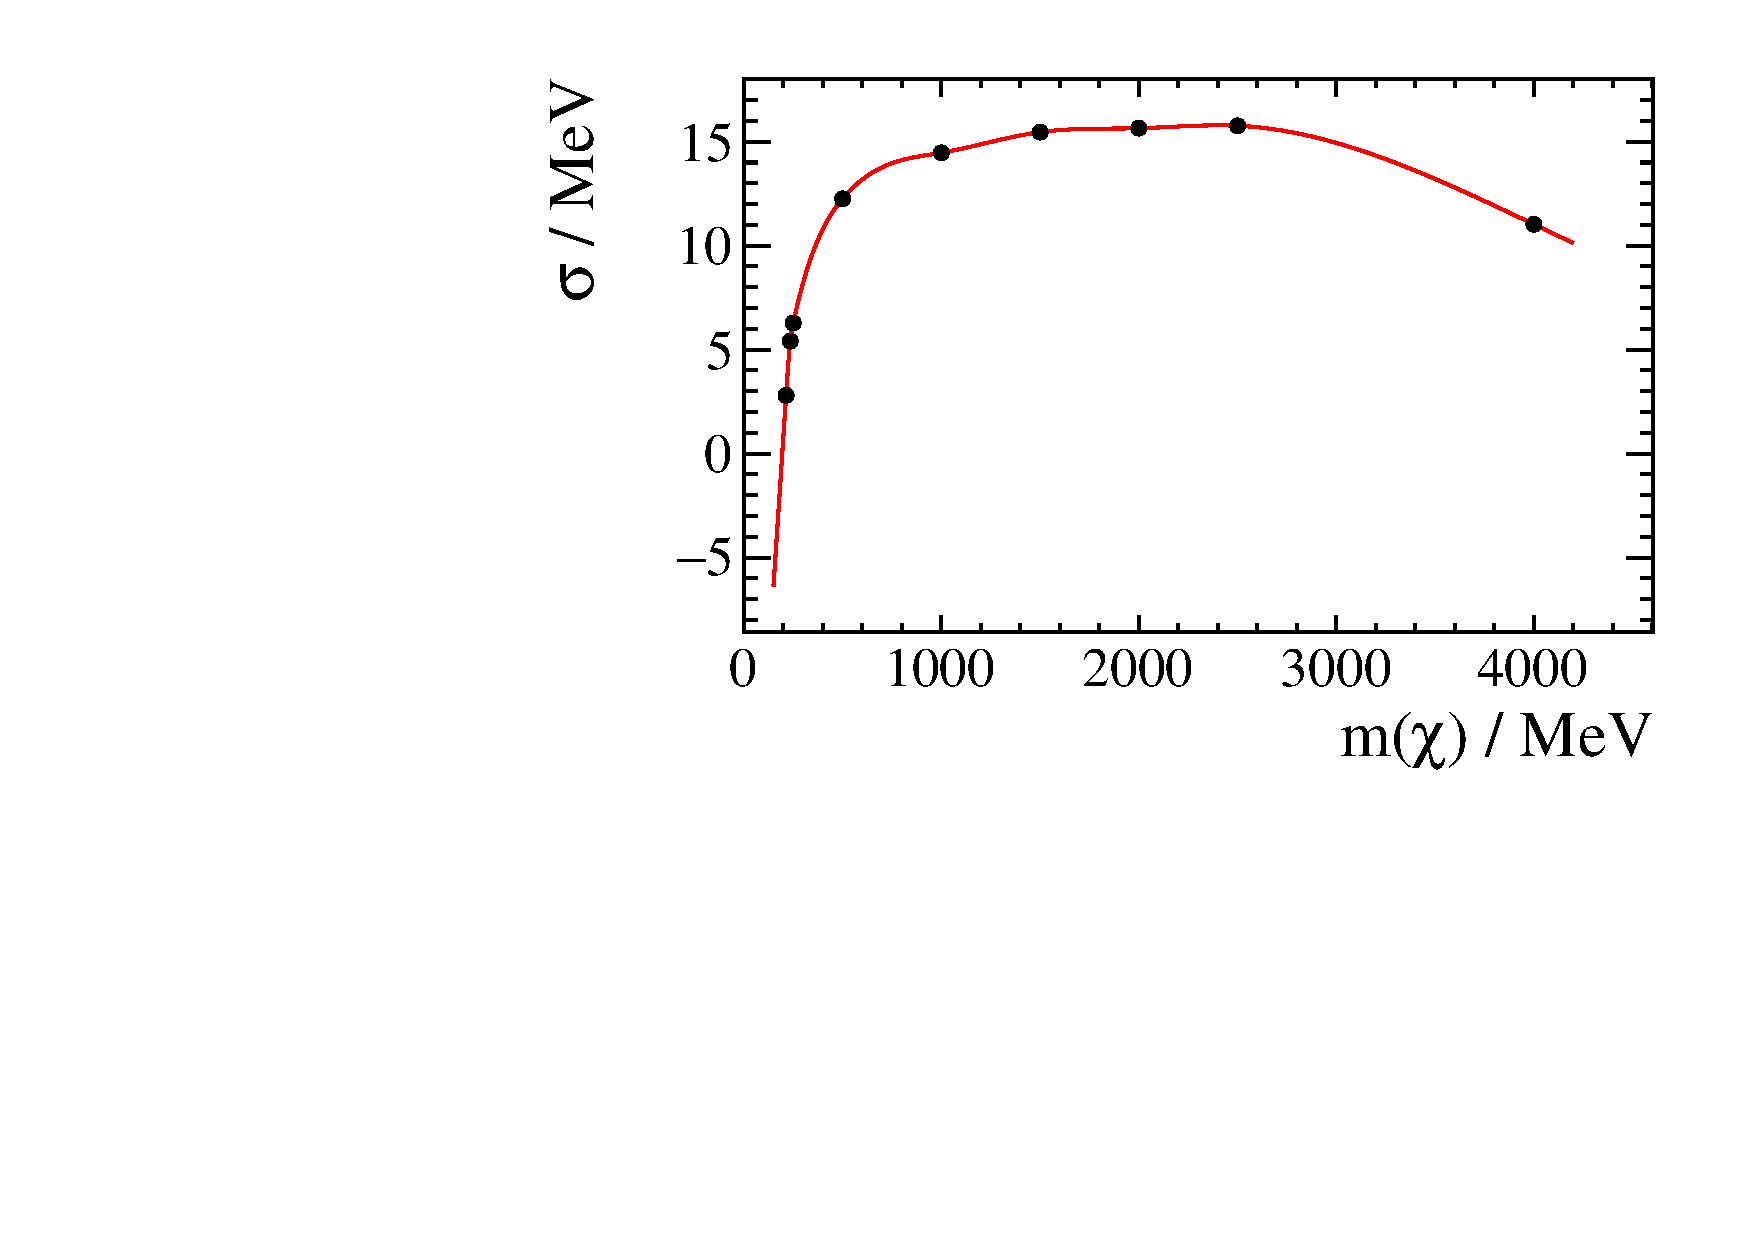
\includegraphics[width=0.48\textwidth]{spline_mass_sig}}
    %\caption{\small
      %Resolutions for the lifetime of a particle as a function of mass in the
      %\protect\subref{fig:eff:spline:res} positive and
      %\protect\subref{fig:eff:spline:resl0} negative directions at the $3\,\sigma$ levets, used to
      %define prompt and displaced regions.
      %\protect\subref{fig:eff:spline:mass} shows the $1\,\sigma$ mass resolution as a function of
      %mass.
      %The black points are from fitted values and the red lines show spline interpolation.
    %}
    %\label{fig:eff:res}
  %\end{center}
%\end{figure}

%%We plan to validate the modeling of this effect in data using some high-statistics decay modes where we have access to kinematical thresholds, {\em e.g.}, \decay{\Bd}{\jpsi K\pi} where the lifetime resolution near the $K\pi$ threshold will be investigated.






%%\subsubsection[A \db produced at threshold]
%%{A $\boldsymbol{\db}$ produced at threshold}
%%In samples of \btokstrdb where $m(\db)=214\mev$ distortions are observed in lifetime resolutions.
%%These manifest themselves in two ways:
%%\begin{itemize}
%%  \item width of resolution larger,
%%  \item on average $\tau_\mathrm{meas}>\tau_\mathrm{true}$.
%%\end{itemize}
%%When the muons are produced so close to the sum of their mass ($2m(\mu) = 211.4$) they are produced
%%with almost no momentum, and therefore their opening angle in the \lhcb detector is very small.
%%This has the effect of merging hits in the \velo and artificially drawing the decay vertex away
%%from the primary vertex; thus increasing the measured lifetime of the \db.
%%The same effect can be seen in MC for \decay{\Bd}{\Kstarz\mumu} where the dimuon pair has low mass.



%\clearpage
%\subsection{Mass resolution of the \db}
%The dimuon mass resolution varies as a function of $m_\mumu$.
%The resolution for each simulated sample is found by fitting the mass spectrum to a
%double Gaussian function.
%The width of a distribution defines the resolution for a given mass, and spline interpolation is again used to obtain the resolution for all $m_\mumu$.
%Figure~\ref{fig:massres} shows the individual fits, while Fig.~\ref{fig:eff:spline:mass} shows
%the mass resolution as a function of mass.


%\begin{figure}
  %\begin{center}
    %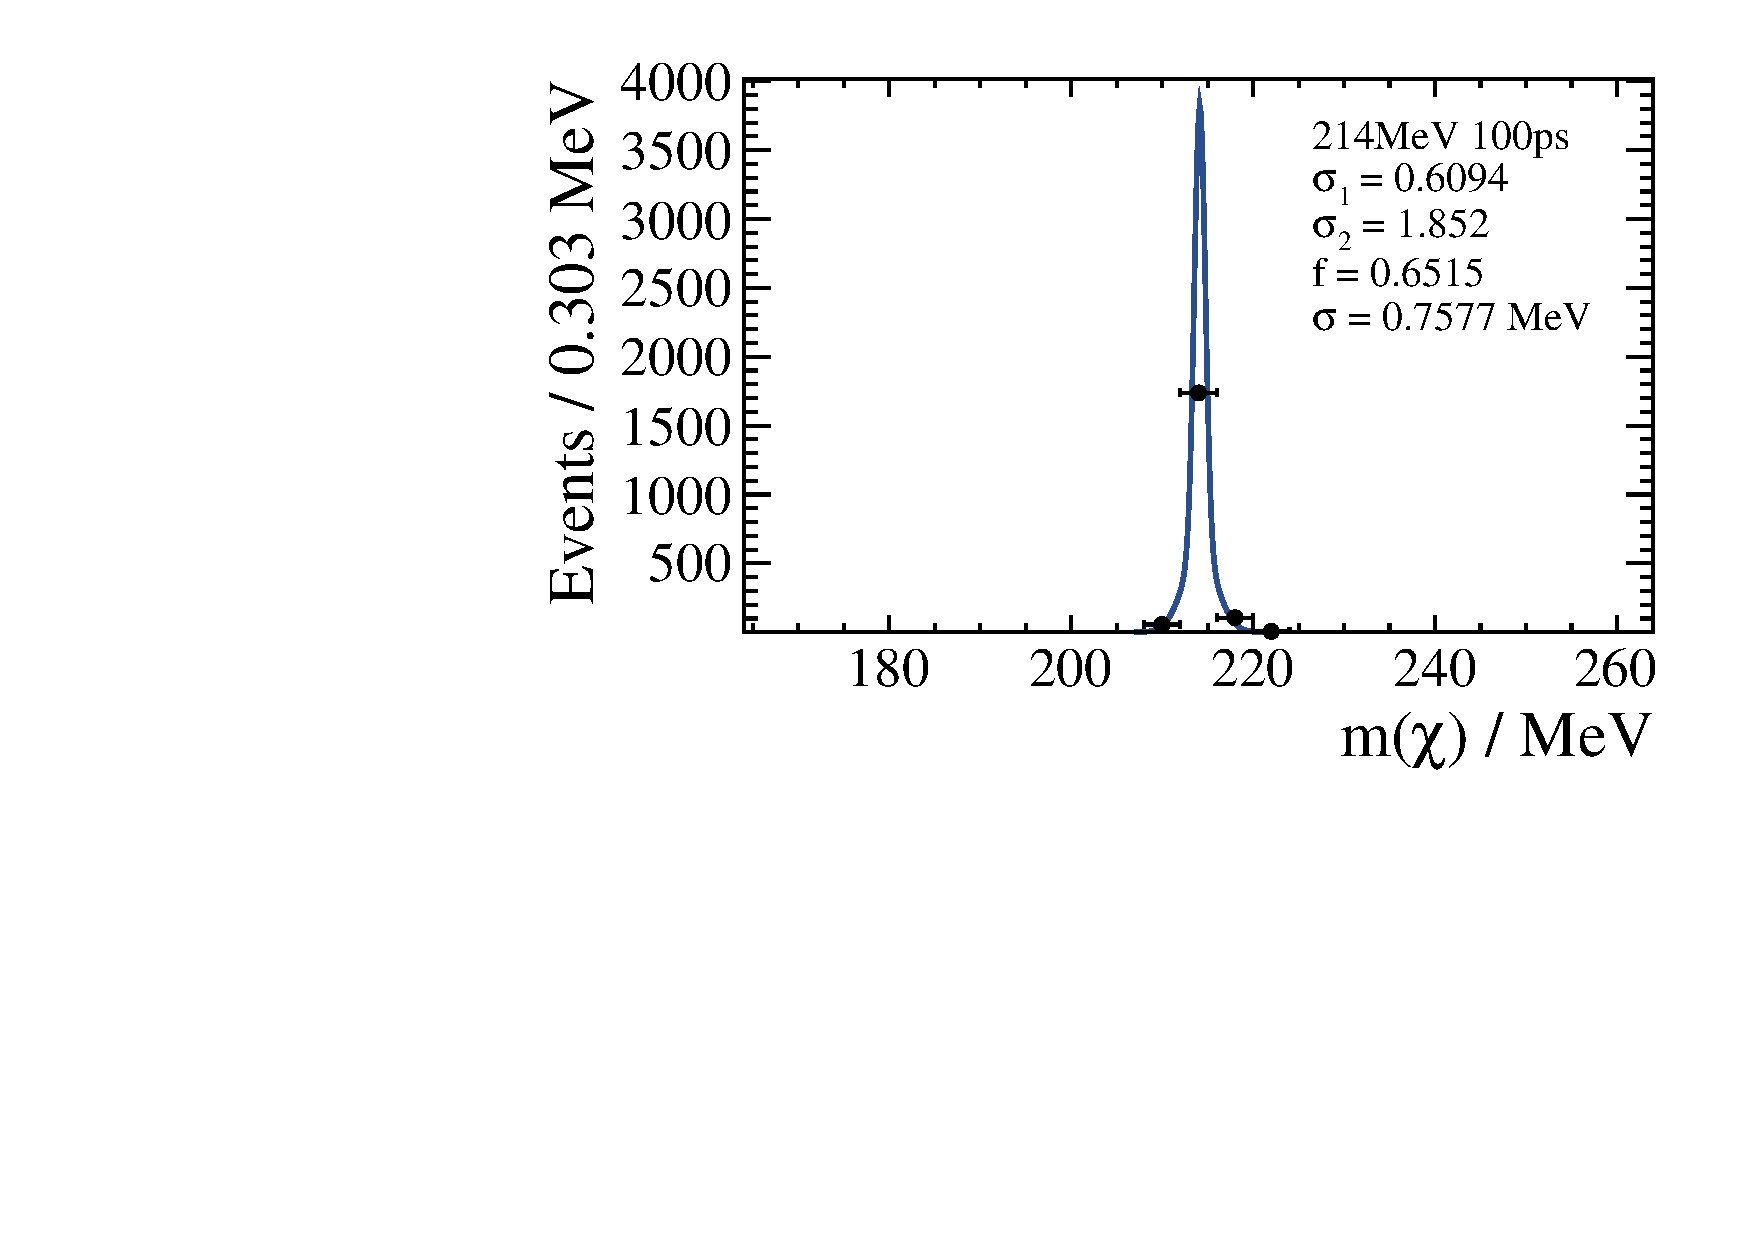
\includegraphics[width=0.42\textwidth]{anaResMass_214_100}
    %%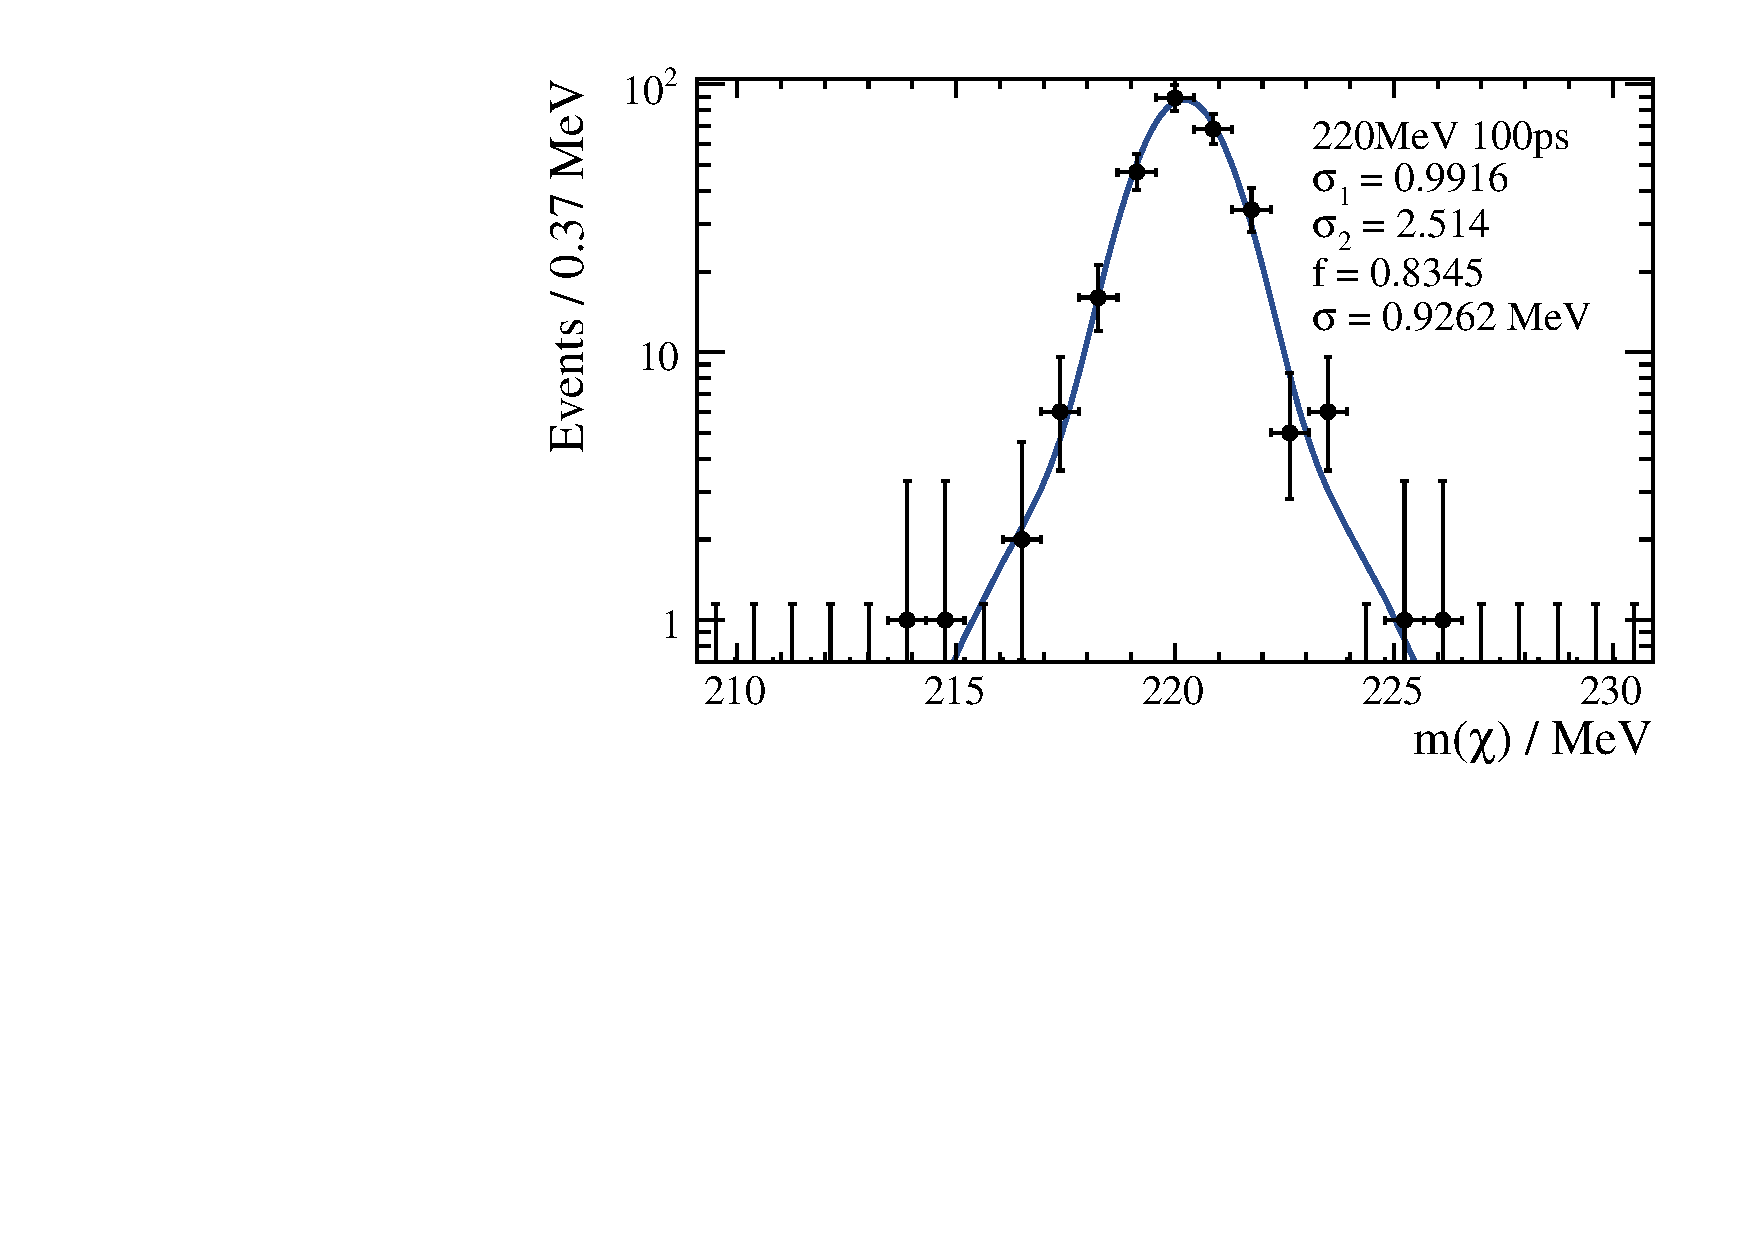
\includegraphics[width=0.32\textwidth]{anaResMass_220_100}
    %%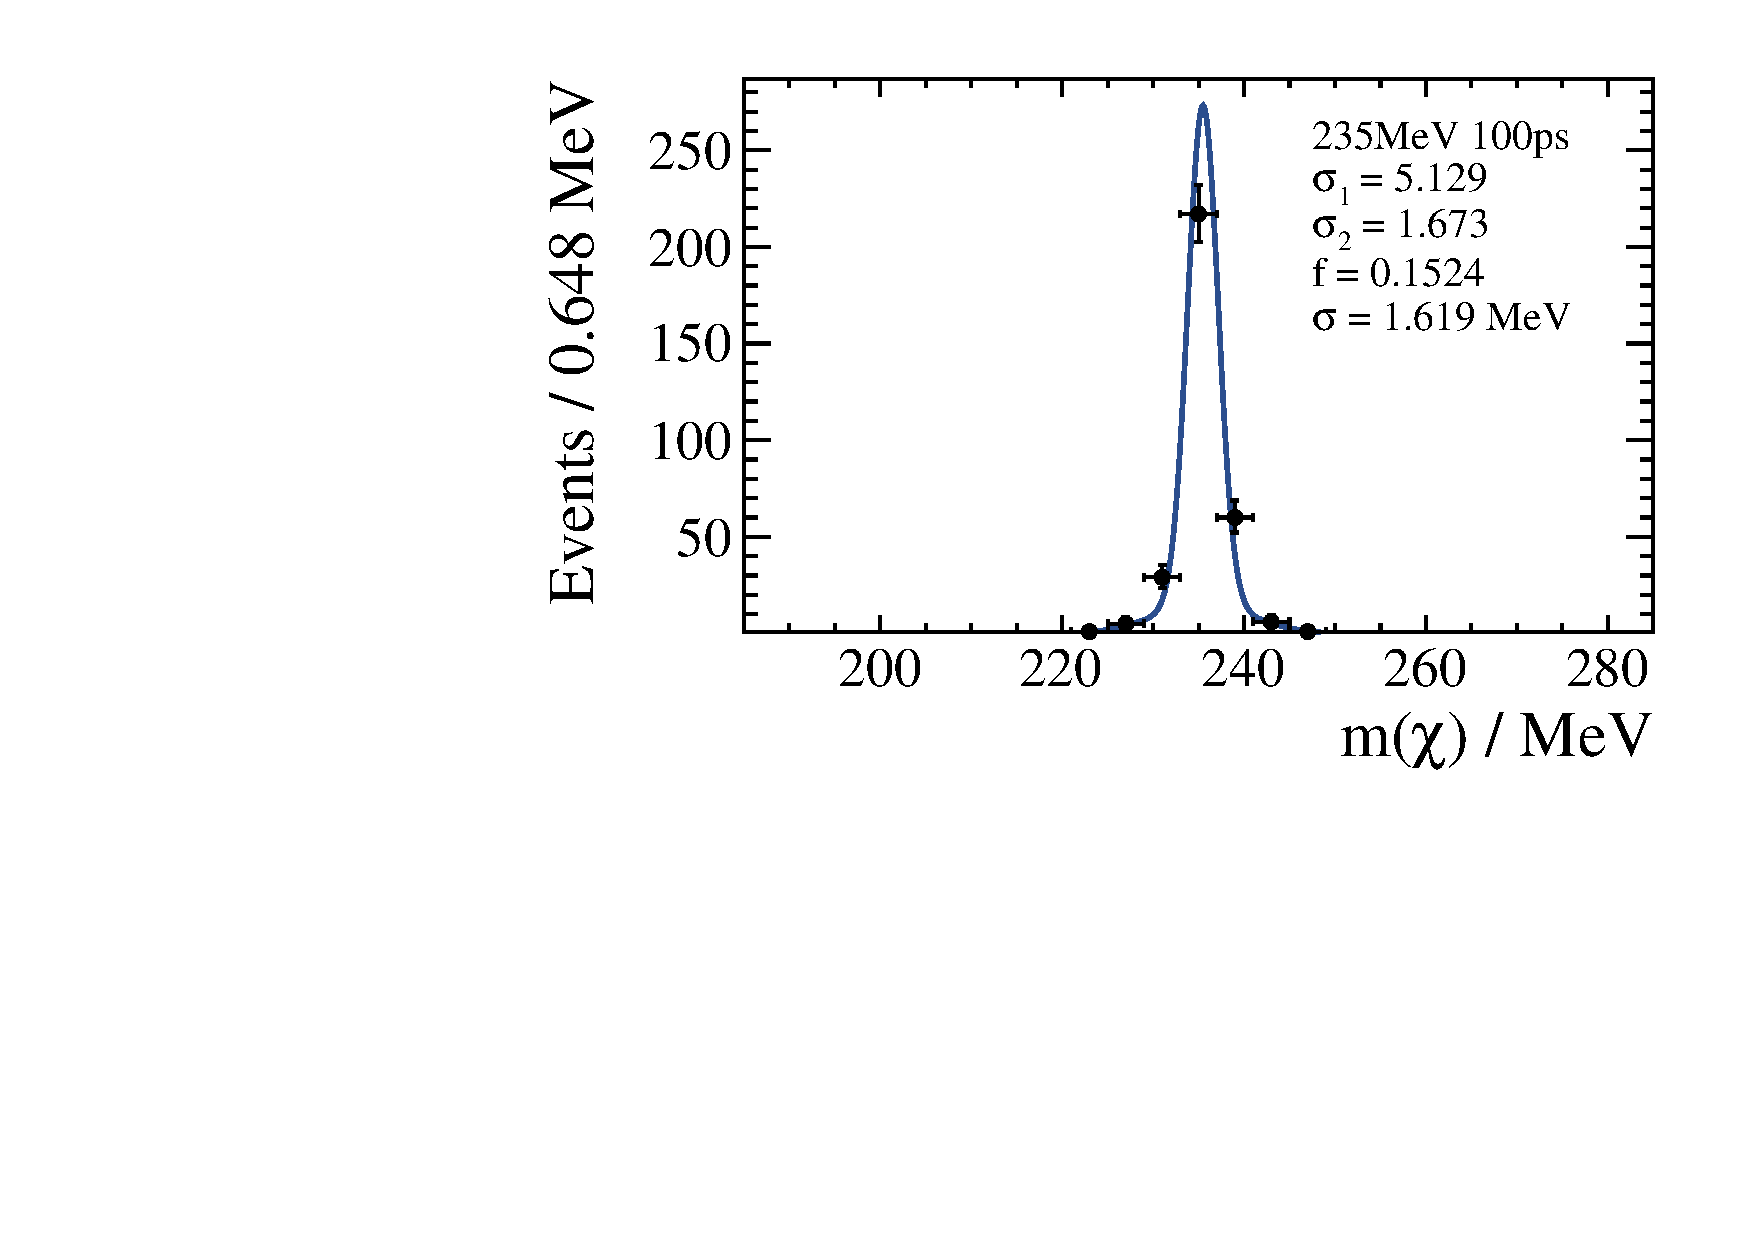
\includegraphics[width=0.32\textwidth]{anaResMass_235_100}
    %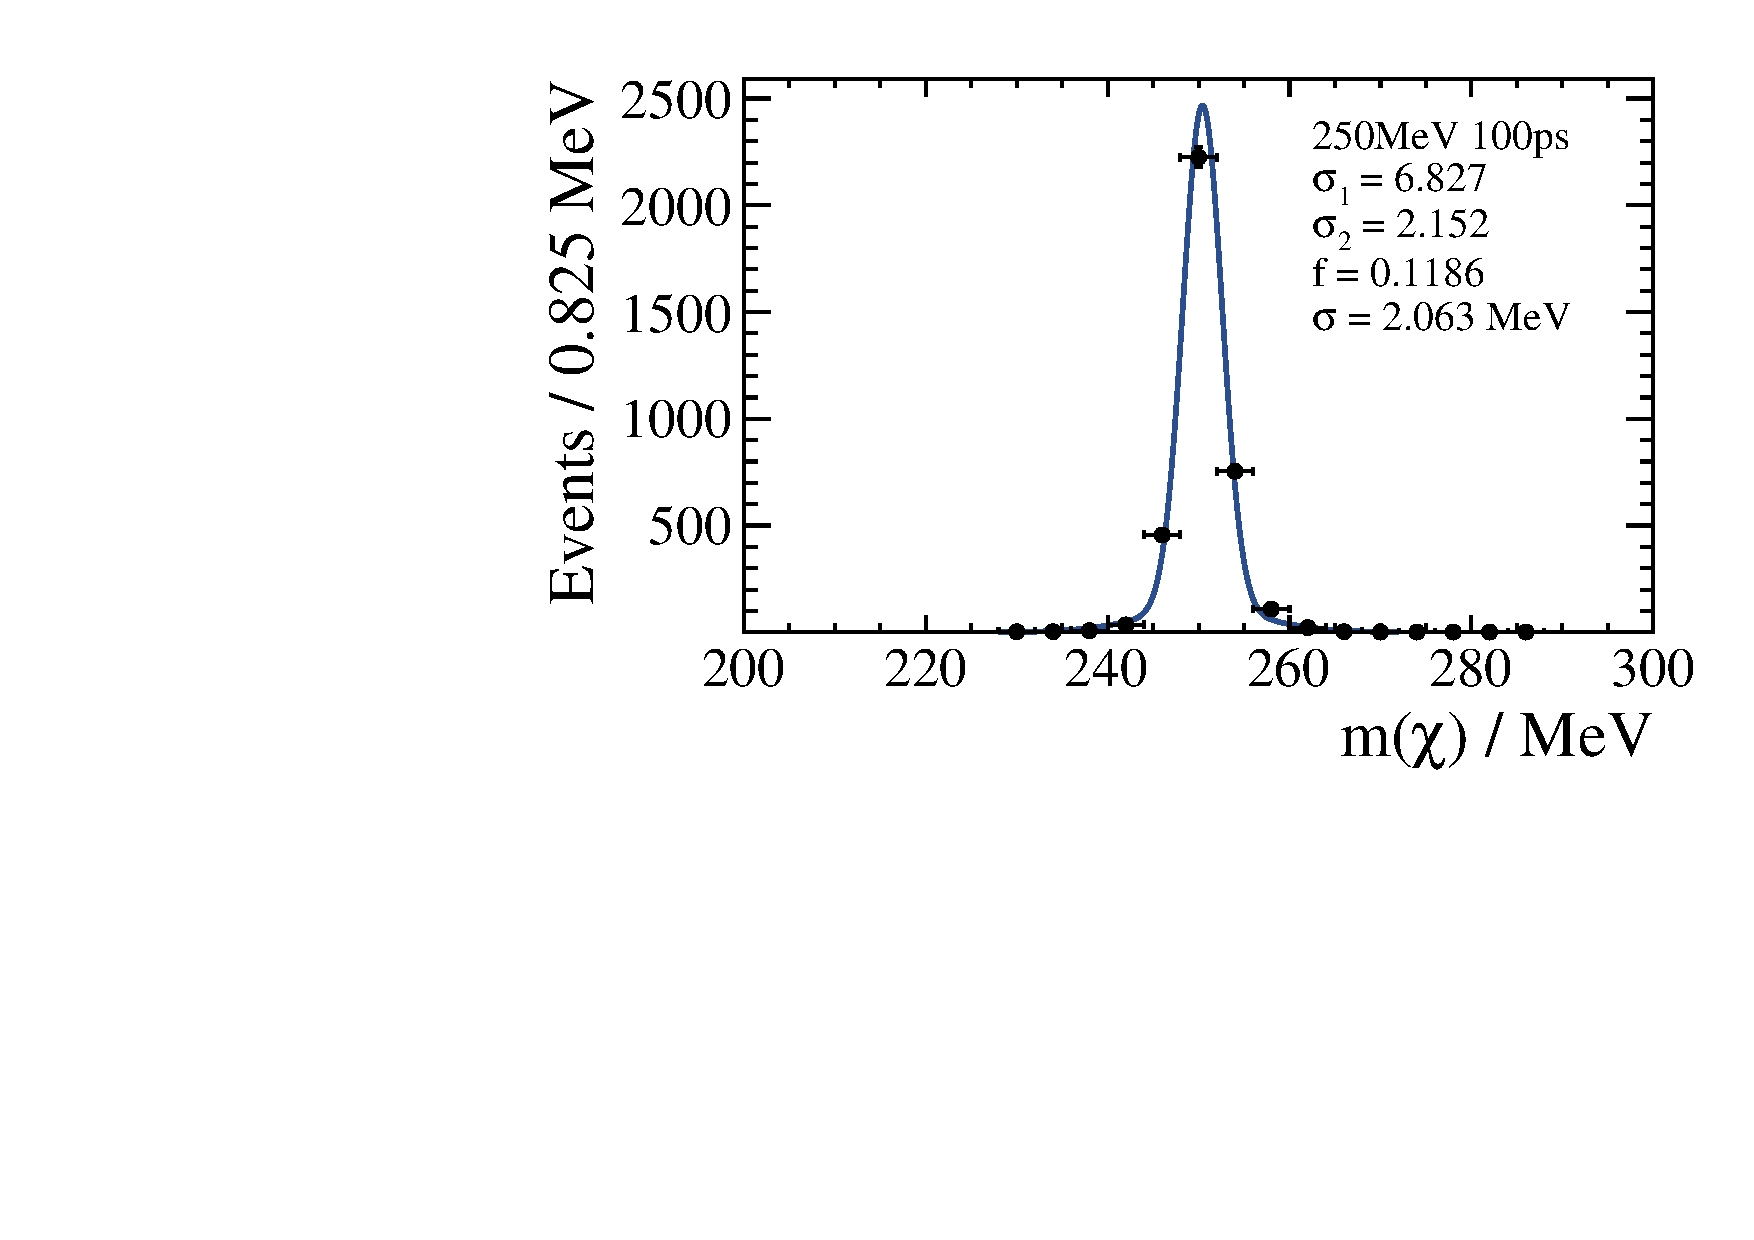
\includegraphics[width=0.42\textwidth]{anaResMass_250_100}
    %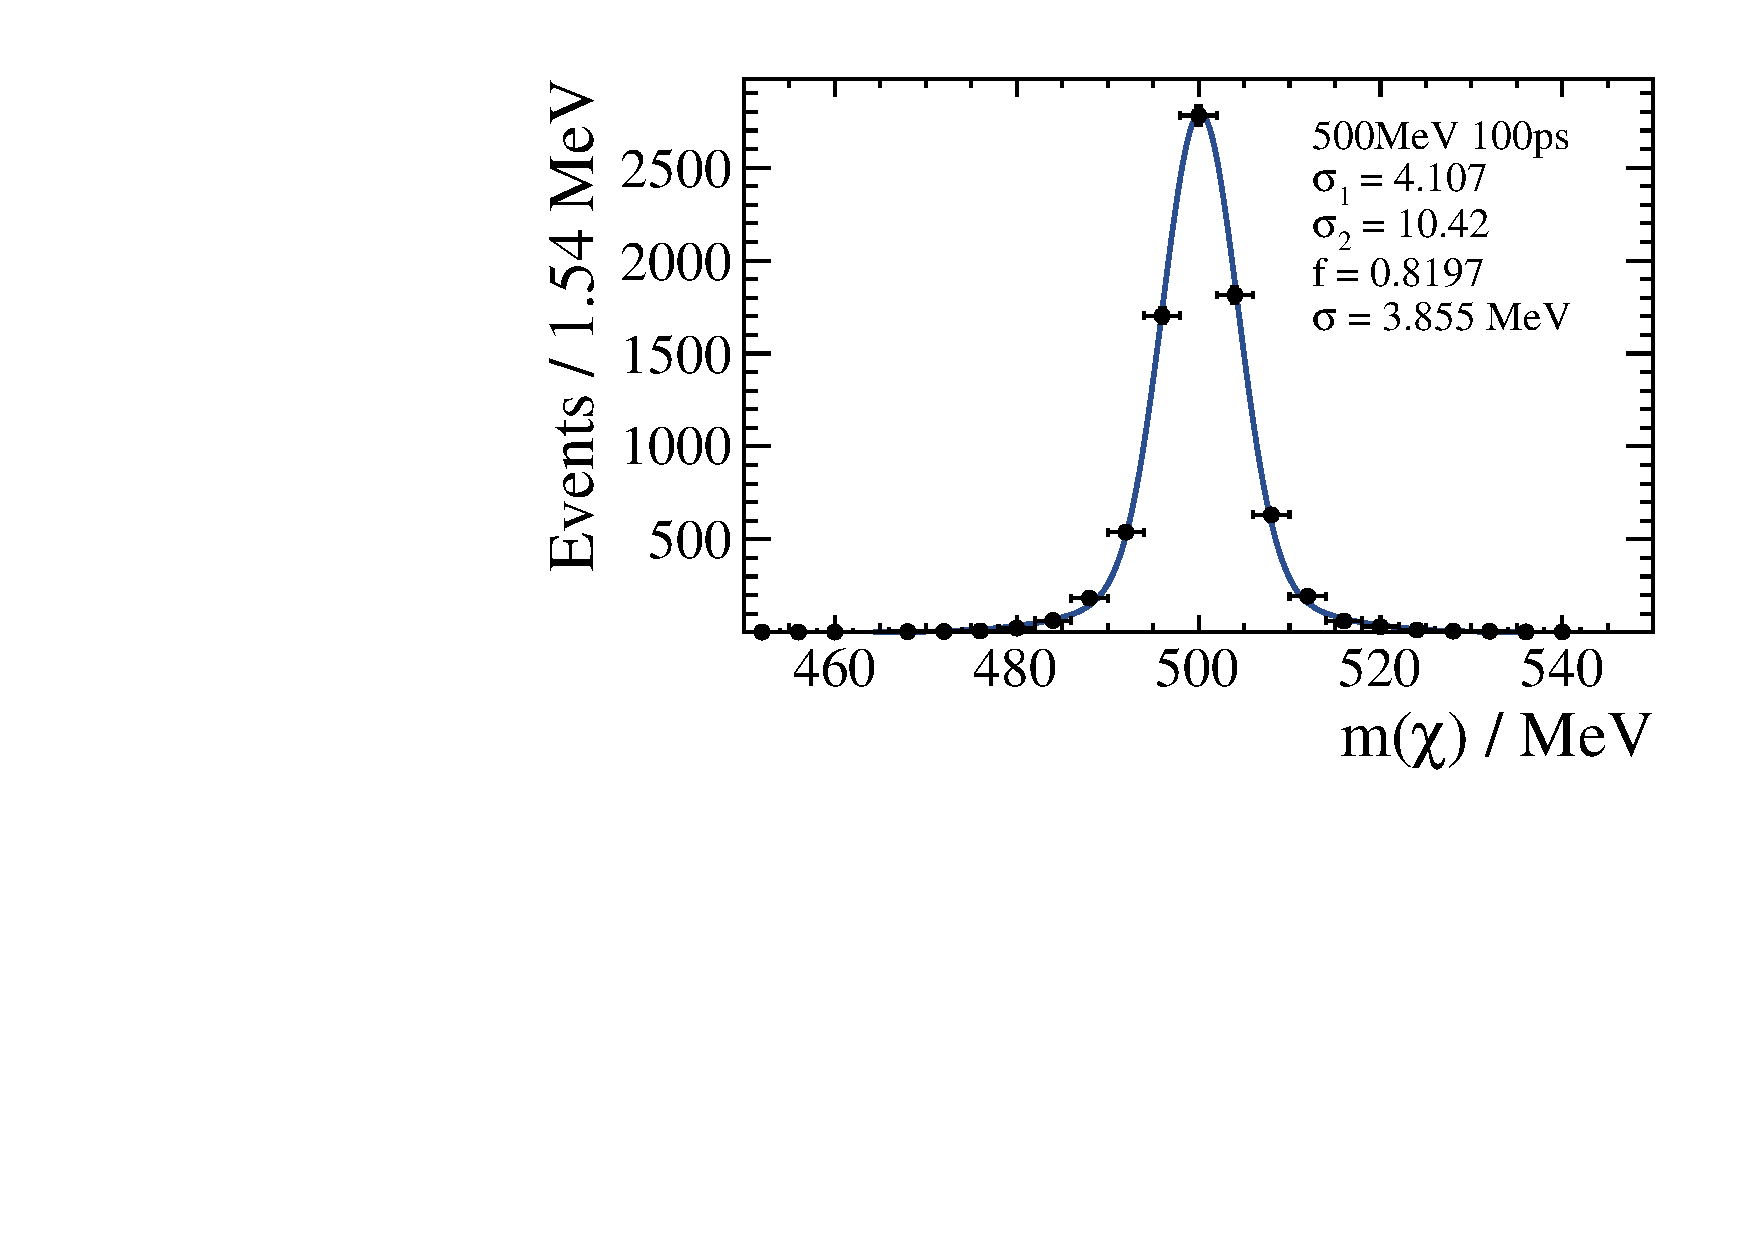
\includegraphics[width=0.42\textwidth]{anaResMass_500_100}
    %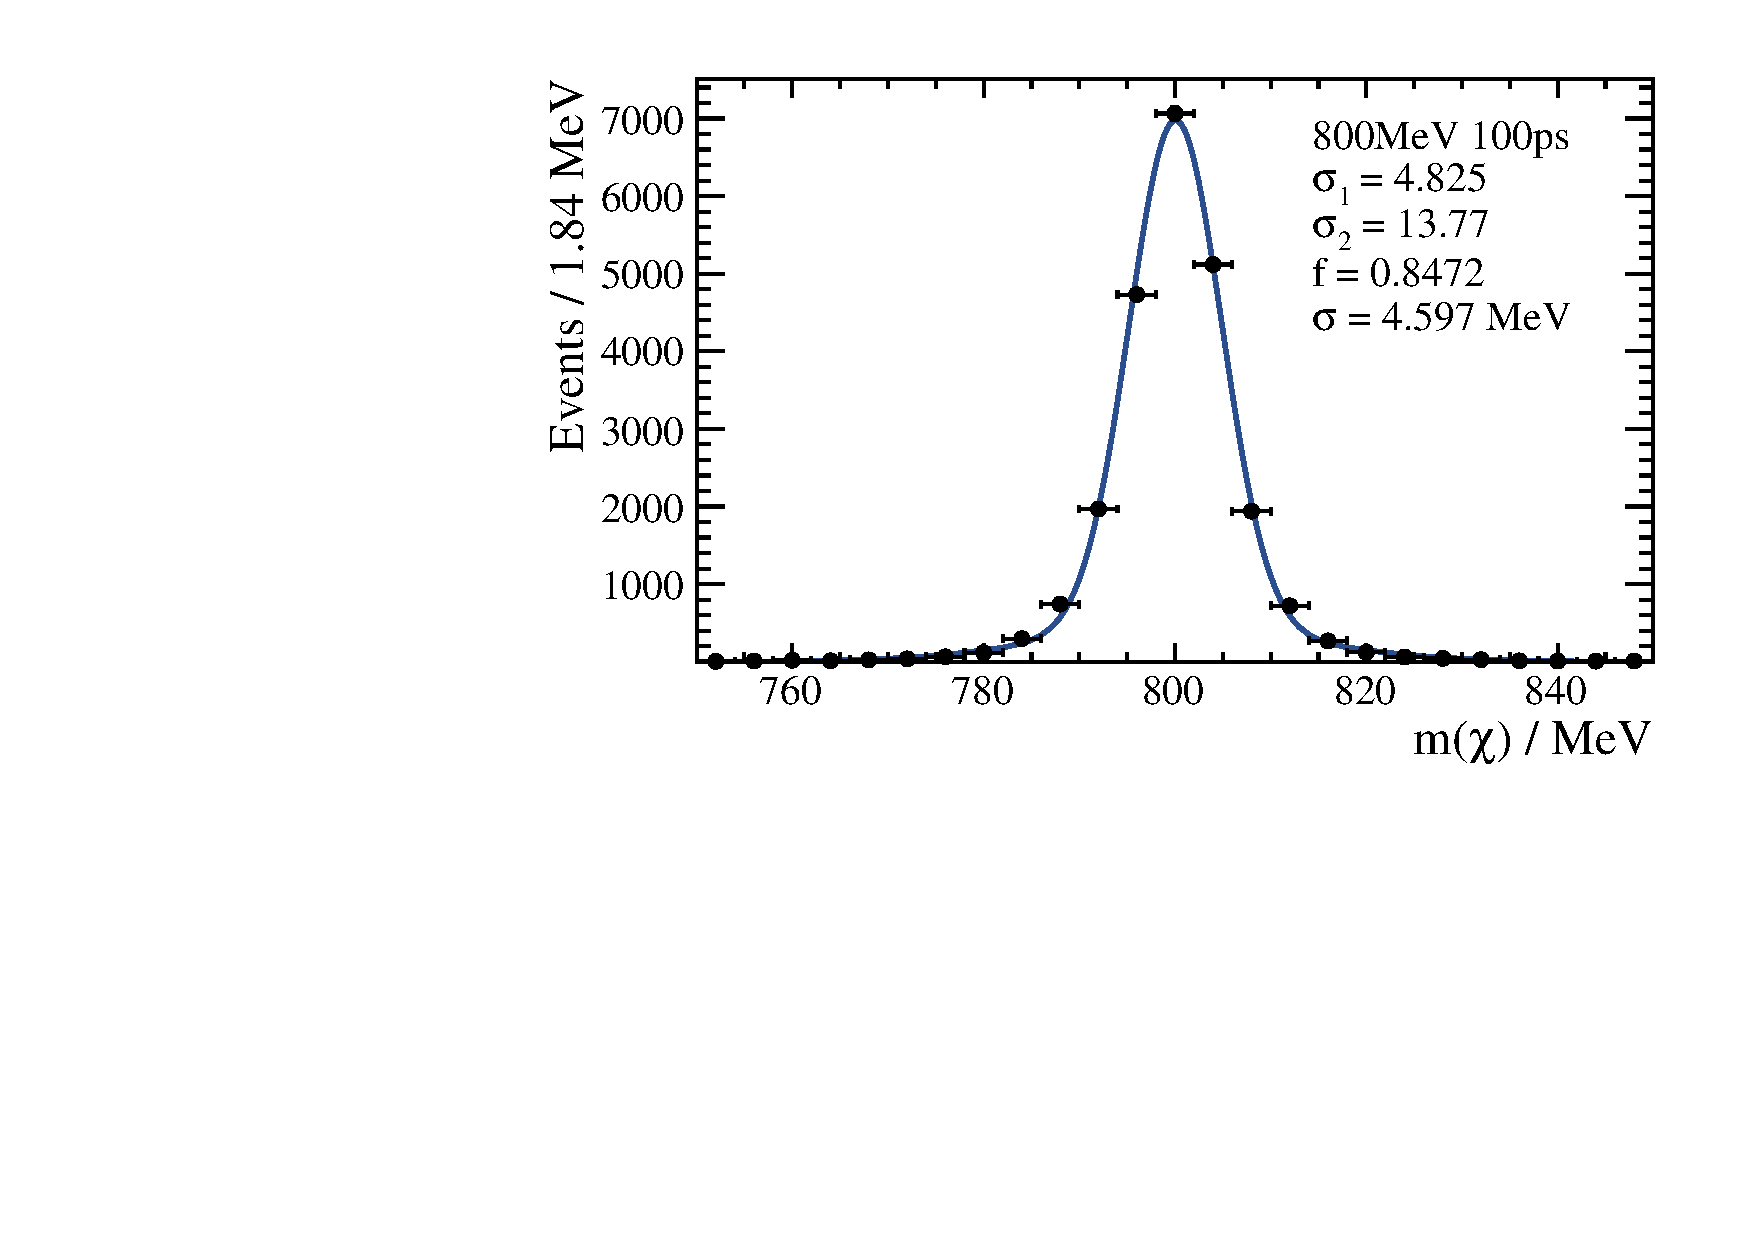
\includegraphics[width=0.42\textwidth]{anaResMass_800_100}
    %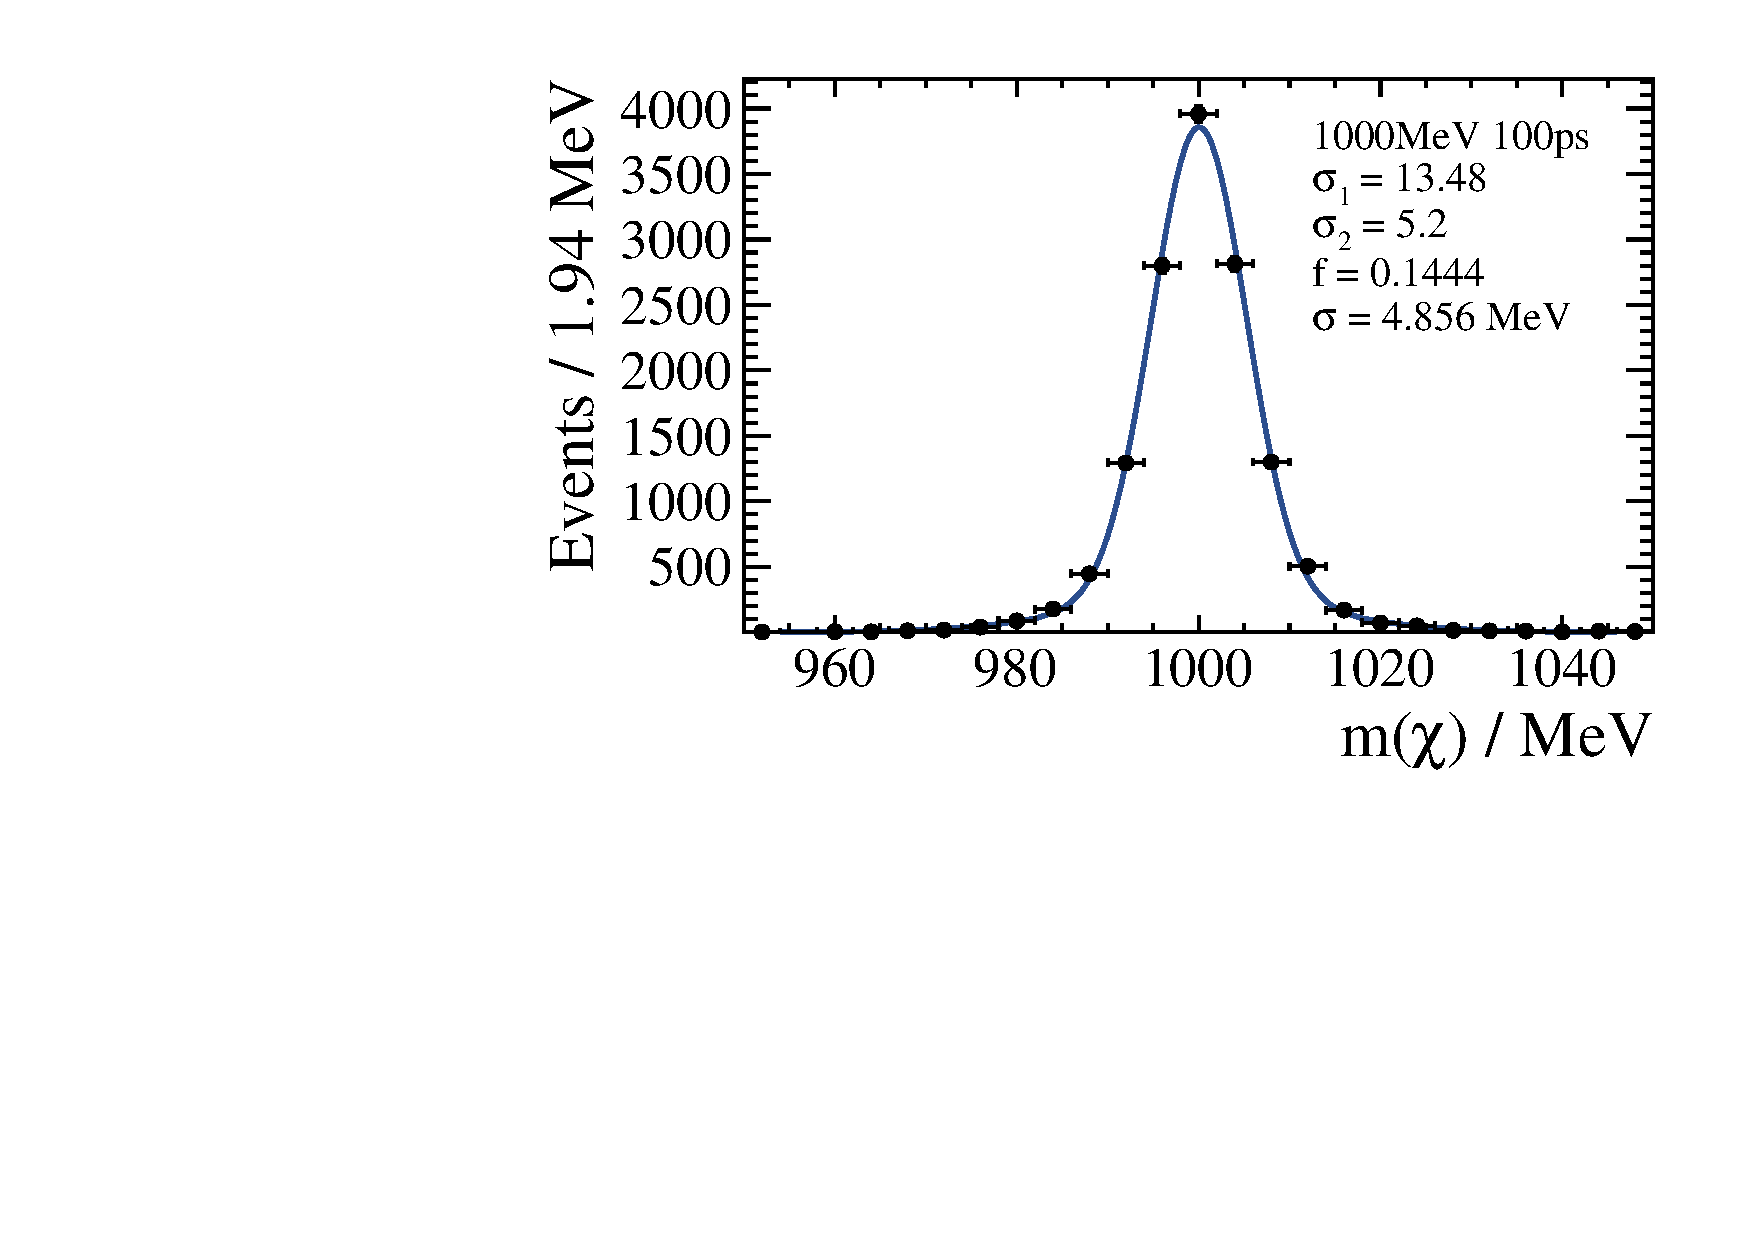
\includegraphics[width=0.42\textwidth]{anaResMass_1000_100}
    %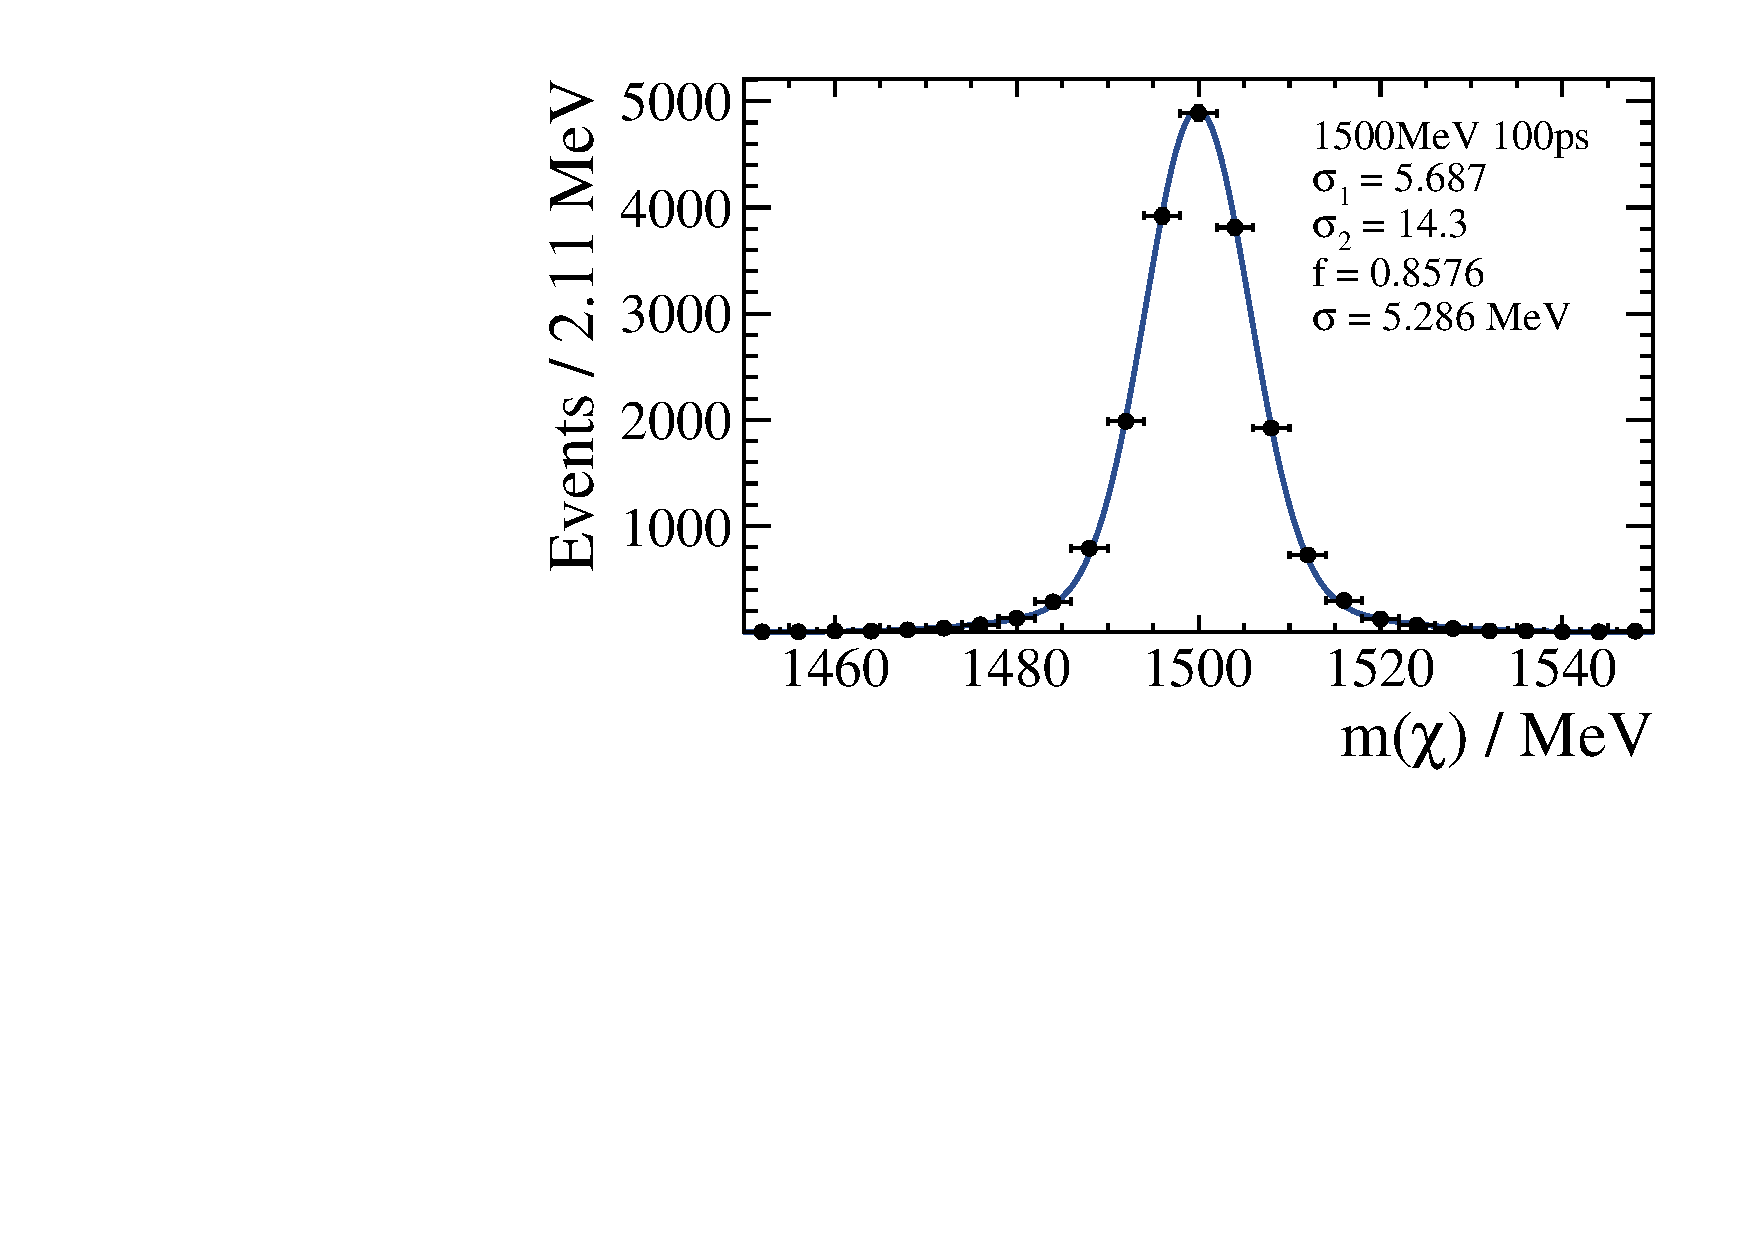
\includegraphics[width=0.42\textwidth]{anaResMass_1500_100}
    %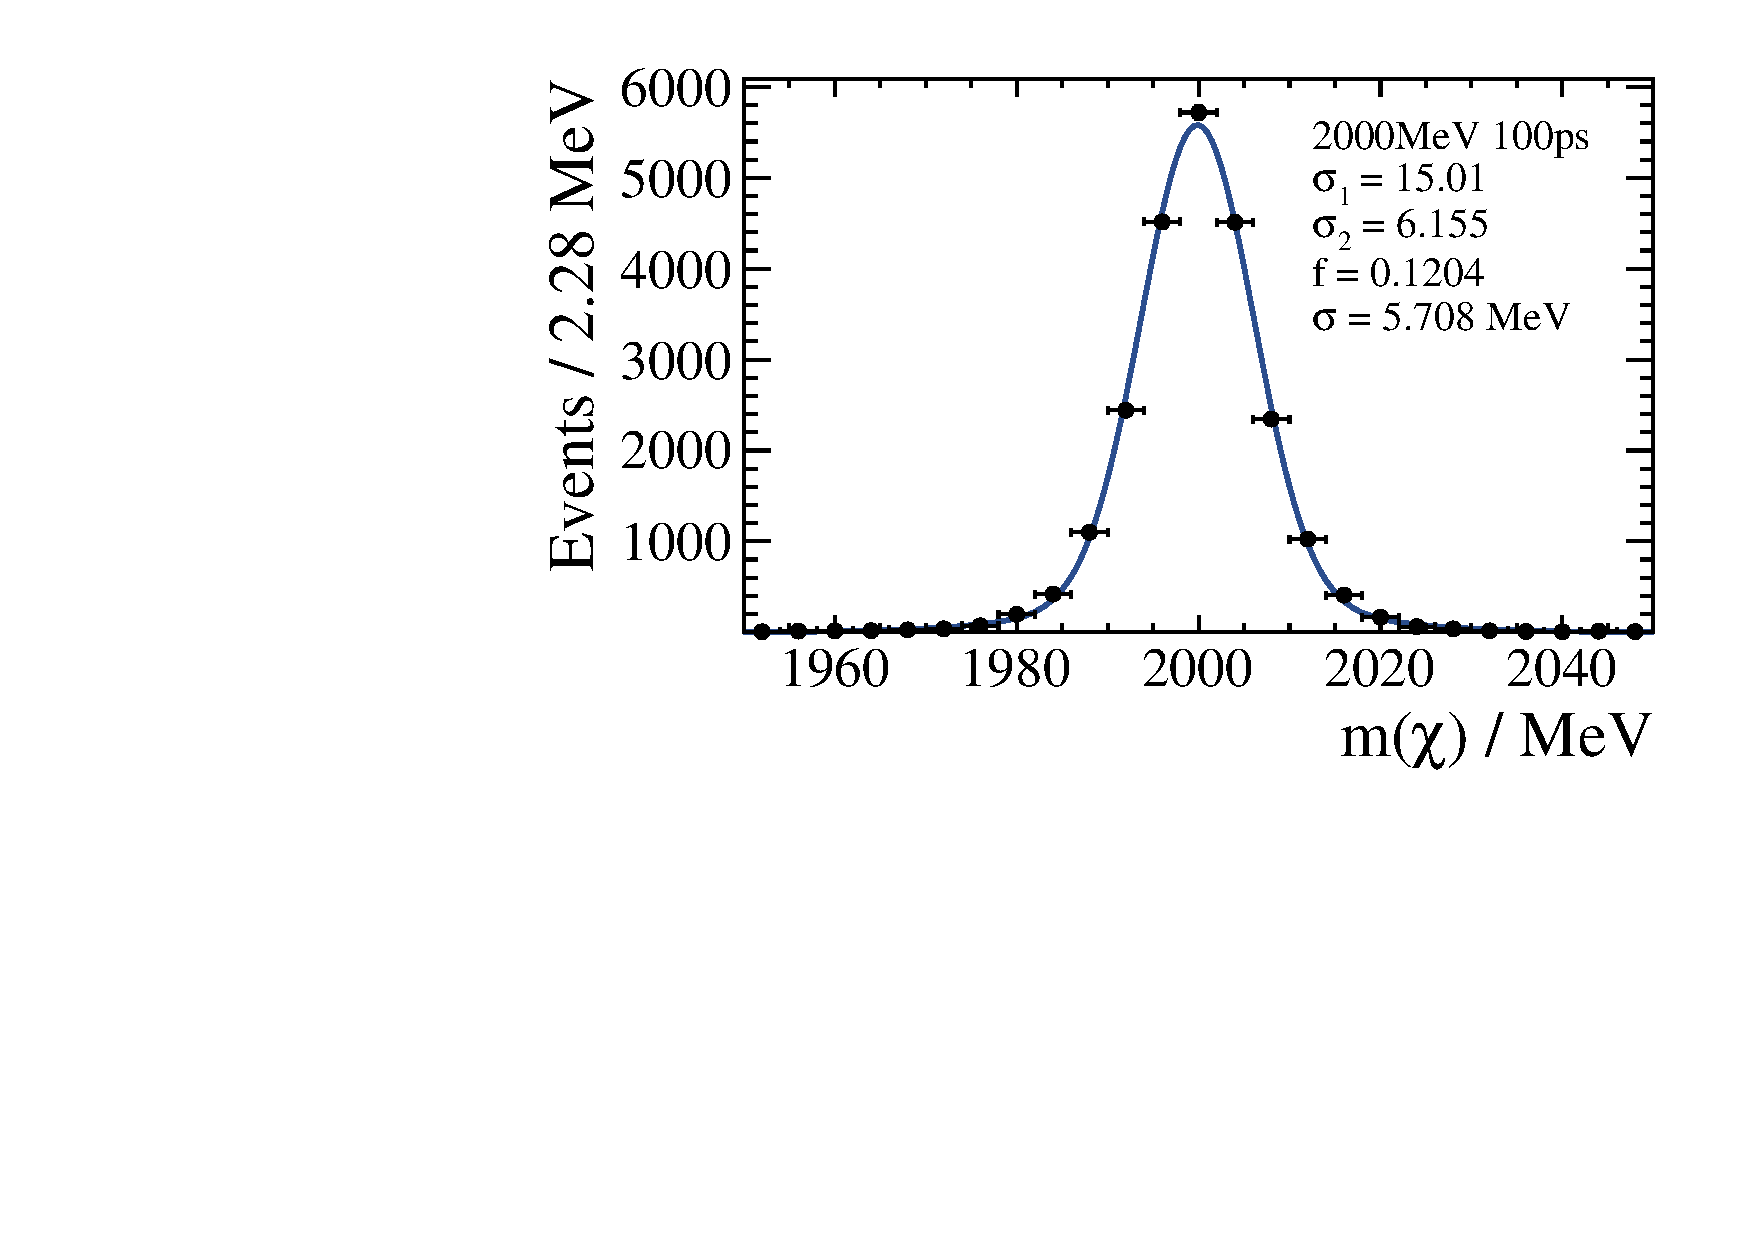
\includegraphics[width=0.42\textwidth]{anaResMass_2000_100}
    %\includegraphics[width=0.42\textwidth]{anaResMass_2500_100}
    %\includegraphics[width=0.42\textwidth]{anaResMass_4000_100}
  %\end{center}
  %\caption{\small
    %Mass resolution for different values of \mdb, each dataset is fit to a double Gaussian
    %function.
  %}
  %\label{fig:massres}
%\end{figure}


%\subsection{Parameterizing the efficiency of the \db selection}
%The shape of the lifetime efficiency distribution varies with mass.
%At each simulated mass point, the lifetime distribution was parameterized with a simple function,
%\begin{equation}
  %\mathcal{T}(\tau) = f\mathcal{G}(\mu, \sigma) + (1-f)\exp\left(-\alpha\tau\right),
  %\label{eq:eff:parameters}
%\end{equation}
%where the parameters depends on dimuon mass.
%This parameterisation is shown fitted to the lifetime distribution of four mass points in
%\Fig{fig:eff:fits}.


%\begin{figure}
  %\begin{center}
    %\subfloat[\label{fig:eff:fit0}]{\includegraphics[width=0.48\textwidth]{anaTauEff_250}}
    %\subfloat[\label{fig:eff:fit1}]{\includegraphics[width=0.48\textwidth]{anaTauEff_800}}\\
    %\subfloat[\label{fig:eff:fit2}]{\includegraphics[width=0.48\textwidth]{anaTauEff_2500}}
    %\subfloat[\label{fig:eff:fit3}]{\includegraphics[width=0.48\textwidth]{anaTauEff_4000}}
    %\caption{\small
      %Fits, using the function in Eq.~\protect\ref{eq:eff:parameters},
      %to the lifetime distributions of simulated events produced with a mass of
      %\protect\subref{fig:eff:fit0} 250,
      %\protect\subref{fig:eff:fit1} 800,
      %\protect\subref{fig:eff:fit2} 2500, and
      %\protect\subref{fig:eff:fit3} $4000\mev$,
      %each with $\tau=100\ps$.
      %The black points are the simulated events, and the black line is the total fit, with light
      %and dark red lines showing the Gaussian and exponential components, respectively.
    %}
    %\label{fig:eff:fits}
  %\end{center}
%\end{figure}


%Samples with different masses are fit with the results for each parameter plotted against dimuon
%mass in \Fig{fig:eff:spline}.
%Extrapolation to different masses is done using spline interpolation, as shown in
%\Fig{fig:eff:spline}.
%The value of $f$ has large errors, and has little effect on the total shape.
%A cubic spline models this very poorly because of the fluctuations at low mass, therefore linear
%regression is used instead.
%These splines account for all efficiencies except for the efficiency of the uBDT and the geometric
%acceptance of the \lhcb detector; the uBDT and geometric acceptance are nearly the same for all
%samples and so nearly cancel in the limit setting.
%An example of a lifetime efficiency distribution for a given mass is shown in \Fig{fig:eff:effmap},
%as is the two-dimensional projection, absolute efficiencies have not been included in this.

%The efficiency map shown in \Fig{fig:res:mbvtau} was generated using simulated samples where
%$\tau(\db)=100\ps$ but contains the efficiency at each $\tau$ below 100\ps.
%It is then possible to obtain the efficiency for any other lifetime as follows:
%\begin{equation}
  %\varepsilon(\tau) = \frac{1}{\tau}\int\limits_0^{100\ps} {\rm d}\tau^{\prime} \mathcal{T}(\tau^{\prime}){\rm exp}(-\tau^{\prime}/\tau),
%%  \left.\exp\left(-\frac{\tau}{x}\right)\right/
%%  \exp\left(-\frac{\tau}{100\ps}\right),
%\end{equation}
%%where $x$ is the `target' lifetime, in ps.
%The upper lifetime acceptance will be $100\ps$, this is because the efficiency for longer lifetimes
%is very poor.


%\begin{figure}
  %\begin{center}
    %\subfloat[\label{fig:eff:spline:sigma}]{\includegraphics[width=0.48\textwidth]{spline_sigma}}
    %\subfloat[\label{fig:eff:spline:alpha}]{\includegraphics[width=0.48\textwidth]{spline_alpha}}\\
    %\subfloat[\label{fig:eff:spline:frac}]{\includegraphics[width=0.48\textwidth]{spline_frac}}
    %%\subfloat[\label{fig:eff:spline:res}]{\includegraphics[width=-2.32\textwidth]{spline_res}}
    %%\subfloat[\label{fig:eff:spline:mass}]{\includegraphics[width=0.32\textwidth]{spline_mass}}
    %\caption{\small
      %%Parameters and mass resolution as a funtion of mass.
      %Parameters from Eq.~\protect\ref{eq:eff:parameters} as a function of mass from
      %simulated events.
      %The parameters are
      %\protect\subref{fig:eff:spline:sigma} $\sigma$,
      %\protect\subref{fig:eff:spline:alpha} $\alpha$, and
      %\protect\subref{fig:eff:spline:frac} $f$.
      %Cubic splines are used to parameterize each shape, except for the parameter $f$, where a
      %linear fit is used.
      %%Parameters $\sigma$, $f$ and $\alpha$ (see Eq.~\protect\ref{eq:eff:parameters})
      %%as a function of $m(\infl)$.
      %%The points are taken from fits to MC, and the adjoining lines show spline interpolation.
    %}
    %\label{fig:eff:spline}
  %\end{center}
%\end{figure}

%\begin{figure}
  %\begin{center}
    %\includegraphics[width=0.48\textwidth]{spline_2d}
    %\caption{\small
      %Using the parameters in Fig.~\ref{fig:eff:spline} and Eq.~\protect\ref{eq:eff:parameters} the
      %lifetime distributions are formed for the full two-dimensional projection.
      %Absolute efficiencies are not folded in here.
    %}
    %\label{fig:eff:effmap}
  %\end{center}
%\end{figure}












